% Options for packages loaded elsewhere
\PassOptionsToPackage{unicode}{hyperref}
\PassOptionsToPackage{hyphens}{url}
\PassOptionsToPackage{dvipsnames,svgnames,x11names}{xcolor}
%
\documentclass[
  12pt,
]{book}
\usepackage{amsmath,amssymb}
\usepackage{iftex}
\ifPDFTeX
  \usepackage[T1]{fontenc}
  \usepackage[utf8]{inputenc}
  \usepackage{textcomp} % provide euro and other symbols
\else % if luatex or xetex
  \usepackage{unicode-math} % this also loads fontspec
  \defaultfontfeatures{Scale=MatchLowercase}
  \defaultfontfeatures[\rmfamily]{Ligatures=TeX,Scale=1}
\fi
\usepackage{lmodern}
\ifPDFTeX\else
  % xetex/luatex font selection
\fi
% Use upquote if available, for straight quotes in verbatim environments
\IfFileExists{upquote.sty}{\usepackage{upquote}}{}
\IfFileExists{microtype.sty}{% use microtype if available
  \usepackage[]{microtype}
  \UseMicrotypeSet[protrusion]{basicmath} % disable protrusion for tt fonts
}{}
\makeatletter
\@ifundefined{KOMAClassName}{% if non-KOMA class
  \IfFileExists{parskip.sty}{%
    \usepackage{parskip}
  }{% else
    \setlength{\parindent}{0pt}
    \setlength{\parskip}{6pt plus 2pt minus 1pt}}
}{% if KOMA class
  \KOMAoptions{parskip=half}}
\makeatother
\usepackage{xcolor}
\usepackage[margin=3cm]{geometry}
\usepackage{longtable,booktabs,array}
\usepackage{calc} % for calculating minipage widths
% Correct order of tables after \paragraph or \subparagraph
\usepackage{etoolbox}
\makeatletter
\patchcmd\longtable{\par}{\if@noskipsec\mbox{}\fi\par}{}{}
\makeatother
% Allow footnotes in longtable head/foot
\IfFileExists{footnotehyper.sty}{\usepackage{footnotehyper}}{\usepackage{footnote}}
\makesavenoteenv{longtable}
\usepackage{graphicx}
\makeatletter
\def\maxwidth{\ifdim\Gin@nat@width>\linewidth\linewidth\else\Gin@nat@width\fi}
\def\maxheight{\ifdim\Gin@nat@height>\textheight\textheight\else\Gin@nat@height\fi}
\makeatother
% Scale images if necessary, so that they will not overflow the page
% margins by default, and it is still possible to overwrite the defaults
% using explicit options in \includegraphics[width, height, ...]{}
\setkeys{Gin}{width=\maxwidth,height=\maxheight,keepaspectratio}
% Set default figure placement to htbp
\makeatletter
\def\fps@figure{htbp}
\makeatother
\setlength{\emergencystretch}{3em} % prevent overfull lines
\providecommand{\tightlist}{%
  \setlength{\itemsep}{0pt}\setlength{\parskip}{0pt}}
\setcounter{secnumdepth}{5}
\usepackage{booktabs}
\ifLuaTeX
  \usepackage{selnolig}  % disable illegal ligatures
\fi
\usepackage[]{natbib}
\bibliographystyle{apalike}
\IfFileExists{bookmark.sty}{\usepackage{bookmark}}{\usepackage{hyperref}}
\IfFileExists{xurl.sty}{\usepackage{xurl}}{} % add URL line breaks if available
\urlstyle{same}
\hypersetup{
  pdftitle={CHAPTER 9: ANALYSIS OF HOUSEHOLD SURVEY DATA},
  pdfauthor={Andrés Gutiérrez, Pedro Luis do Nascimento Silva},
  colorlinks=true,
  linkcolor={blue},
  filecolor={Maroon},
  citecolor={Blue},
  urlcolor={Blue},
  pdfcreator={LaTeX via pandoc}}

\title{CHAPTER 9: ANALYSIS OF HOUSEHOLD SURVEY DATA}
\author{Andrés Gutiérrez\footnote{Comisión Económica para América Latina y el Caribe (CEPAL) - \href{mailto:andres.gutierrez@cepal.org}{\nolinkurl{andres.gutierrez@cepal.org}}}, Pedro Luis do Nascimento Silva\footnote{SCIENCE, \href{mailto:pedronsilva@gmail.com}{\nolinkurl{pedronsilva@gmail.com}}}}
\date{2024-11-08}

\begin{document}
\maketitle

{
\hypersetup{linkcolor=}
\setcounter{tocdepth}{0}
\tableofcontents
}
\listoffigures
\listoftables
\hypertarget{abstract}{%
\chapter*{Abstract}\label{abstract}}
\addcontentsline{toc}{chapter}{Abstract}

Analyzing complex household survey data requires knowing and properly applying the foundations of the design-based inference. The researcher will be faced to a small database that contains specific information that will allow her to make conclusions over the whole population.

The purpose of any analysis on this kind of datasets is not referred to make conclusions on the sample itself -- which in most of the cases is a small subgroup of the population - but to the domains of interest and the whole population. Having that into account, the first step in any analysis plan should be devoted to defining the sampling design based on the selection mechanisms used to draw the final sample and the findings on the field related to nonresponse and lack of coverage.

The chapter covers three main topics of analysis: descriptive statistics; comparisons and association; and modeling of survey data. On the one hand, we introduce simple descriptive statistics, such as totals, frequencies, means and proportions, quantiles and some graphics; on the other, we delve deeper on complex relationships between the variables of the survey. All these analyses rely on the representativity principle of the design-based inference. This way, the reader will find a strong focus, not only on point estimates, but also on uncertainty measures. The chapter also presents a short discussion on the different approaches that can be used to estimate variances; the best way to visualize the estimates; and NSO practical experiences.

\hypertarget{introduction}{%
\chapter*{Introduction}\label{introduction}}
\addcontentsline{toc}{chapter}{Introduction}

A key concern of every agency that produces statistical information is with the \emph{correct} use of the data that it produces. This is even reflected in the United Nations \emph{Fundamental Principles of Official Statistics}, namely:

\begin{itemize}
\item
  \textbf{Principle 3.} To facilitate a correct interpretation of the data, the statistical
  agencies are to present information according to scientific standards on the sources,
  methods and procedures of the statistics.
\item
  \textbf{Principle 4.} The statistical agencies are entitled to comment on erroneous
  interpretation and misuse of statistics.
\end{itemize}

Here we emphasize a particular aspect, aiming to empower users when analysing household survey data. The computer revolution, with the resulting ease of access computers, created favorable conditions for the increased use of statistical data, including those resulting from household sample surveys. Sometimes this data is used for purely descriptive purposes. Other times, however, its use is made for analytical purposes, involving the testing of hypothesis or the construction of models, when the objective is to draw conclusions that are also applicable to populations other than the one from which the sample was extracted. In such cases, standard statistical software may provide biased or misleading results. This chapter's purpose is to present the relevant models, methods and software to enable users to account for the complex survey design frequently used to conduct household sample surveys when analysing the resulting data.

What makes such data special for those who intend to use them for analytical purposes?
The answer is that they are obtained through complex sample surveys of finite populations that often involve: \emph{stratification}, \emph{clustering} of units of analysis, \emph{unequal probabilities of selection}, and \emph{weighting adjustments} to compensate for non-response and/or improve precision.

Standard data analysis methods and software typically ignore these aspects, and may produce biased estimates of both the target parameters and the variances of these estimates. In this chapter we analyze the impact of simplifications made when using standard data analysis methods and software, and present the necessary adjustments to these procedures in order to appropriately incorporate the aspects highlighted here into the analysis.

In section 9.1, a short discussion on the fundamental principles of the design-based inference is presented, emphasizing that conclusions taken from probability sample surveys should be based on a pair: the point estimate and it associated margin of error (or any related measure). In section 9.2, we begin the journey with simple descriptive statistics: means, ratios, proportions and other typical descriptive parameters. Section 9.3 is devoted to more complex parameters that allow comparisons of the phenomenon of interest between subgroups for continuous and discrete variables. In this section we present standard tests to compare means and measure the degree of association between variables, and also consider the problem of correlation and association. Section 9.4 focuses on modelling survey outcomes. We first involve the reader in an discussion on the role of weighting when estimating regression coefficients. Then, we introduce some proper approaches to estimate complex parameters in linear and logistic regression models. Finally, section 9.5 presents a summary of ideas and tools for survey data visualization showing the best practices for creating graphics and maps in a context where uncertainty measures of estimates are important.

Most of the sections in the chapter present national experiences that will guide the reader on how NSOs are dealing with the different stages of the analysis of household survey data.

The purpose of this chapter is defining and explaining basic concepts of the design-based paradigm in household surveys to analyze complex household survey data. In section 9.1, a short discussion on the fundamental principles of the design-based inference is presented, emphasizing that conclusions taken from this kind of surveys should be based on a pair: the point estimate and it associated margin of error (or any related measure). In section 9.2, we begin the journey with simple descriptive statistics: means, ratios, proportions and other parameters are part of this discussion. Section 9.3 is devoted to more complex parameters that allow comparisons of the phenomenon of interest between subgroups for continuous and discrete variables. In this section we present standard tests to compare means and measure the degree of association between variables. This section also deals with the problem of correlation and association. Section 9.4 focuses on modelling survey outcomes. We first involve the reader in an discussion on the role of weighting when estimating regression coefficients. Then, we introduce some proper approaches to estimate complex parameters in linear and logistic regression models. Finally, section 9.5 presents a summary on survey data visualization showing the best practices for creating graphics and maps in a context where uncertainty measures of estimates are important.

Most of the sections in the chapter present national experiences that will guide the reader on how currently NSOs are dealing with the different stages of the analysis of household survey data.

\hypertarget{the-golden-pair-sample-design-and-estimator}{%
\chapter{The golden pair: sample design and estimator}\label{the-golden-pair-sample-design-and-estimator}}

Accounting for the sampling design is crucial for analyzing complex survey data. We must ensure that PSU, strata, and weights are available in the survey dataset to enable adequate analysis. Alternatively, when such information is not available, the dataset should at least contain replicate weights, or the analyst should have clear guidance on how to compute both point and variance estimates.

A well-described survey design facilitates statistical analysis, supports effective data interpretation, and enables meaningful insights into complex phenomena. Missing or incorrect design information may lead to biased estimates and misleading conclusions.

\hypertarget{parameters-and-estimators}{%
\section{Parameters and estimators}\label{parameters-and-estimators}}

Under a design-based approach this section presents the basic principles of inductive inference and how, using the \emph{sampling weights} (from chapter VIII), one can get consistent estimators for population parameters of interest. We adopt the notation introduced in chapter VIII for presenting the expressions required here.

The \emph{population total} \(Y = \sum _{U} y_k\) and \emph{mean} \(\overline Y = \frac Y N\) of a survey variable \(y\) can be estimated by weighted estimators given by \(\widehat Y _{HT} = \sum _{s} d_k \ y_k\) and \(\overline y_{H} = \frac {\widehat Y_{HT}} {\widehat N_{HT}} = \frac {\sum_{s} d_k \ y_k} {\sum_{s} d_k}\), respectively. When the survey weights are calibrated and/or non-response adjusted, the above expressions may still be used, but with the calibrated or non-response adjusted weights, \(w_k\) say, replacing the design weights \(d_k\), for all \(k \in s\).

Here \(s = \left\{ k_1, \ldots, k_n \right\} \subset U\) denotes the set of units in a sample selected from the population \(U\) using a \emph{probability sampling design} \(p(s)\), that ensures strictly positive first order inclusion probabilities \(\pi_k = Pr(k \in s), \, \forall \, k \in U\). These inclusion probabilities are assumed known \(\forall \, k \in s\), at least to the data producers.

Under the design-based framework and assuming full response, \(\widehat Y _{HT}\) is unbiased for \(Y\) and its sampling variance is given by

\[
V_p \left( \widehat{Y}_{HT} \right) = \sum_{k \in U} \sum_{j \in U} \left( \frac {d_k d_j} {d_{kj}} - 1 \right) y_k y_j
\]

where \(d_{kj} = 1 / \pi_{kj}\) and \(\pi_{kj} = Pr(k,j \in s), \, \forall \, k,j \in U\). This result assumes that the sampling design \(p(s)\) is such that \(\pi_{kj} > 0 \,\, \forall \, k,j \in U\).

Under full response, this variance can be estimated unbiasedly by

\[
\widehat {V_p} \left( \widehat{Y}_{HT} \right) = \sum_{k \in s} \sum_{j \in s} \left( d_k d_j - d_{kj} \right) y_k y_j
\]

While the above formula for variance estimation is general and covers the vast majority of sample designs used in the practice of household sample surveys, it is not used in practice because the second order inclusion probabilities \(\pi_{kj}\) (and corresponding pairwise weights \(d_{kj}\)) are generally unknown to survey data analysts. In fact, even data producers do not compute such pairwise weights, since there are more efficient methods for variance estimation that do not require having such weights.

\hypertarget{uncertainty-in-household-surveys}{%
\section{Uncertainty in household surveys}\label{uncertainty-in-household-surveys}}

As the sample is typically a small subset of the population, it is important to obtain not only point estimates for the parameters of interest, but also the corresponding uncertainty measures and/or confidence intervals. In this subsection we present some approaches for variance estimation: approximate formulas from \emph{Taylor linearization} and/or the \emph{ultimate cluster} approach for variances under multi-stage cluster sampling. We also introduce replication methods and generalized variance functions, which are essential when PSU or strata are missing from the sample dataset.

A unifying idea of sampling theory is that of estimating equations - \citet{Binder1983}. Many population parameters can be written/obtained as solutions for \emph{population estimating equations}. A generic population estimating equation is given by \$\sum\_\{i \in U\} z\_i (\theta) = 0 \$, where \(z_i(\bullet)\) is an \emph{estimating function} evaluated for unit \(i\) and \(\theta\) is a population parameter of interest.

For the case of the population total, take \(z_i(\theta) = y_i - \theta / N\). The corresponding population estimation equation is given by \(\sum _{i \in U} (y_i - \theta / N) = 0\), and solving for \(\theta\) gives the population total \(\theta_U = \sum _{i \in U} y_i \ = \ Y\). Similarly, take \(z_i(\theta) = y_i - \theta\) for the population mean. As a final example, consider the ratio of population totals. Taking \(z_i(\theta) = y_i - \theta x_i\), the corresponding population estimation equation is given by \(\sum _{i \in U} (y_i - \theta x_i) = 0\). Solving for \(\theta\) gives the \emph{population ratio} \(\theta_U = \sum _{i \in U} y_i / \sum _{i \in U} x_i \ = \ R\).

The idea of defining population parameters as solutions to population estimating equations allows defining a general method for obtaining corresponding sample estimators. It is a matter of using the \emph{sample estimating equations} \(\sum _{k \in s} d_k \, z_k (\theta) = 0\). Under \emph{probability sampling}, full response and with \(d_k = 1 / \pi_k\), the sample sum in the left hand side is unbiased towards the population sum in the corresponding population estimating equation. Solving the sample estimating equation yields consistent estimators for the corresponding population parameters.

The case of the population mean yields the sample estimating equation \(\sum _{k \in s} d_k (y_k - \theta) = 0\), and by solving on \(\theta\), we recover the Hàjek estimator \(\widehat \theta = \sum _{k \in s} d_k \, y_k \, / \sum _{k \in s} d_k = \overline y_H\). In the case of the population ratio, solving \(\sum _{k \in s} d_k (y_k - \theta x_k) = 0\) on \(\theta\), yields the well-known estimator \(\widehat \theta = \sum _{k \in s} d_k \, y_k \, / \sum _{k \in s} d_k \, x_k = \widehat R\).

The variance of estimators obtained as solutions of sample estimating equations can be obtained as:

\[
V_p (\widehat \theta) \doteq \left[ J (\theta_U) \right] ^{-1} V_p \left[ \sum _{k \in s} d_k \, z_k (\theta_U) \right] \left[ J (\theta_U) \right] ^{-1}
\]

where \(J (\theta_U) = \sum _{k \in U} \left[ \partial{z_k (\theta)} / \partial \theta \right]_{\theta = \theta_U}\), and \(\theta_U\) is the solution of the corresponding population estimating equation.

A consistent estimator of this variance is given by:

\[
\widehat V_p (\widehat \theta) = \left[ \widehat J ( \widehat \theta) \right] ^{-1} \widehat V_p \left[ \sum _{k \in s} d_k \, z_k (\widehat \theta)\right] \left[ \widehat J ( \widehat \theta) \right] ^{-1}
\]

where \(\widehat J (\widehat \theta) = \sum _{k \in s} d_i \, \left[ \partial{z_k ( \theta)} / \partial \theta \right]_{\theta = \widehat \theta}\).

This approach implies that by one is able to estimate many population parameters and corresponding variances using essentially well known methods for estimating totals. Its simplicity and generality have enabled the development of software such as the \texttt{R\ survey} package, the \texttt{Stata\ svy} functions and others.

\hypertarget{ultimate-cluster-method}{%
\section{Ultimate Cluster Method}\label{ultimate-cluster-method}}

The central idea of the \emph{Ultimate Cluster} method for variance estimation for estimators of totals in multi-stage cluster sampling designs, proposed by \citep{Hansen1953}, is to consider only the variation between information available in the level of PSUs, and assume that these would have been selected with replacement from the PSU population. This idea is simple, but quite powerful, because it allows to accommodate a variety of sampling designs, involving stratification and selection with unequal probabilities (with or without replacement) of both PSUs as well as lower level sampling units. The requirements for the application of this method are that one has unbiased estimators of totals for the variable of interest for each sampled PSU, and that data are available for at least two sampled PSUs in each stratum (if the sample is stratified in the first stage).

Although the method was originally proposed for estimation of variances of estimated totals, it can also be applied in combination with Taylor linearization to obtain variance estimates for estimators of other population quantities that can be obtained as solutions to sample estimating equations.

Consider a multi-stage sampling design, in which \(m_{h}\) PSUs are selected in stratum \(h,\) \(h=1,\ldots ,H\). Let \(\pi_{hi}\) be the inclusion probability of PSU \(i\) stratum \(h\), and by \(\widehat{Y}_{hi}\) an unbiased estimator of the total \(Y_{hi}\) of the survey variable \(y\) for the \(i\)-th PSU in stratum \(h\), \(h=1,\ldots ,H\). Hence an unbiased estimator of the population total \(Y = \sum_{h=1}^{H} \sum_{i \in U_{1h}} Y_{hi}\) is given by \(\widehat{Y}_{UC} = \sum_{h=1}^{H} \sum_{i \in s_{1h}} d_{hi} \widehat{Y}_{hi}\), and the \emph{ultimate cluster} estimator of the corresponding variance is given by:

\[
\widehat{V}_{UC} \left( \widehat{Y}_{UC}\right) = \sum_{h=1}^{H} \frac{m_{h}}
{m_{h}-1} \sum_{i=1}^{n_{h}} \left( d_{hi} \widehat{Y}_{hi} - \frac{\widehat{Y}_{h}}{m_{h}} \right) ^{2}
\]

where \(U_{1h}\) and \(s_{1h}\) are the population and sample sets of PSUs in stratum \(h\), \(d_{hi} = 1 / \pi_{hi}\), \(\widehat{Y}_{h} = \sum_{i=1}^{n_{h}} d_{hi} \widehat{Y}_{hi}\) for \(h=1,\ldots ,H\). (See for example, \citep{Shah1993}, p.~4).

Although often the selection of primary units can have Primary Cluster estimator presented here may provide a reasonable approximation of the corresponding variance of randomization. This is because sampling plans without replacement are generally more efficient than plans with replacement of equal size. Such an approximation is widely used by sampling practitioners to estimate variances of usual descriptive quantities such as totals and medium (with due adaptation) due to their simplicity, compared to the much greater complexity involved with the employment of variance estimators that attempt to incorporate all steps of plans sampling in several stages. A discussion about Quality of this approximation and alternatives can be found in \citep{SSW92}, p.~153.

In some cases, sample replication methods (\emph{bootstrap}, \emph{jackknife}) can also be used to estimate variances, as we will see later.

\hypertarget{bootstrap-method}{%
\section{Bootstrap Method}\label{bootstrap-method}}

The method was proposed by \citet{Efron1979}, but the version we consider here is the so-called Rao-Wu-Yue Rescaling Bootstrap, which is adequate for stratified multi-stage sampling designs commonly used in household surveys - see \citet{Rao1992}. This method is now widely used for variance estimation with complex survey data. To implement this method, you need to follow the sequence of steps outlined below.

Step 1. Select a simple random sample with replacement of size \(m_h - 1\) of PSUs in each of the \(H\) design strata. Each selected PSU takes with it all the subordinate sampling units and their data.

Step 2. Repeat Step 1 \(R\) times, and denote by \(m_{hi}(r)\) the number of times the PSU \(i\) of stratum \(h\) was selected for the sample in replicate \(r\).

Step 3. Calculate the \emph{bootstrap} weight of unit \(k\) within PSU \(i\) of stratum \(h\) as \(w_{hik} (r) = w_{hik} \times \frac {m_h}{m_h - 1} \times m_{hi}(r)\).

Step 4. For each replica \(r\), calculate an estimate \(\widehat \theta_{(r)}\) of the target parameter \(theta\) using the \emph{bootstrap} weights \(w_{hik} (r)\).

Step 5. Estimate the variance using:

\[
\widehat V_{B} \left( \widehat \theta \right) = \frac {1} {R} \sum_{r=1}^R \left( \widehat \theta_{(r)} - \tilde \theta \right)^2
\]

where \(\tilde \theta = \frac 1 R \sum_{r=1}^R \widehat \theta_{(r)}\) is the average of the replica estimates.

Whenever the original sampling weights \(w_{hik}\) receive non-response adjustments or are calibrated, the corresponding non-response adjustments and/or calibration of the basic weights must be repeated for each replica, so that the variance estimates adequately reflect the effects of the calibration and non-response adjusments on the uncertainty of the point estimates.

This method is more computationally costly, but provides good estimates of variance, including for quantiles and other parameters of complex nonlinear forms. It also makes it easier for users who do not have access to software capable of calculating complex variance expressions based on Taylor linearization, etc. The survey package allows you to generate \emph{bootstrap} replicas and also estimate variances using this method.

\hypertarget{using-software-to-generate-valid-inferences}{%
\section{Using software to generate valid inferences}\label{using-software-to-generate-valid-inferences}}

In this part, we advocate to using specialized statistical software to generate efficient estimation processes. Those packages support complex survey data analysis by specifying the survey design using appropriate commands or functions.

\hypertarget{descriptive-parameters}{%
\chapter{Descriptive parameters}\label{descriptive-parameters}}

The most frequent analysis of complex household survey data consists in estimating some descriptive population parameters for a range of survey variables. Such \emph{descriptive analysis} generally involve estimating frequencies, proportions, means, and totals. But other target parameters such as selected quantiles of numeric variables, poverty and inequality measures, and a range of indicators such as those required for monitoring the Sustainable Development Goals are becoming part of regular set of estimates needed from household sample surveys.

\hypertarget{frequencies}{%
\section{Frequencies}\label{frequencies}}

\hypertarget{point-estimation}{%
\subsection{Point Estimation}\label{point-estimation}}

The accurate estimation of absolute sizes and proportions in household surveys is essential for obtaining representative data that reflects the demographic and socioeconomic reality of a population. These figures serve as the basis for public policy decision-making, resource allocation, and the design of social programs.

The ability to understand the distribution of specific categories, such as poverty status, employment status, education level, among others, provides valuable information to address inequalities and promote equitable development.

\hypertarget{size-estimates}{%
\subsection{Size Estimates}\label{size-estimates}}

In this section, the processes for estimating categorical variables will be carried out. First, one of the most important parameters is the size of a population, which represents the cardinality of that set; in other words, the total number of individuals that comprise it. In terms of notation, the population size is estimated as follows:

\[
\widehat{N} = \sum_{h=1}^{H} \sum_{i \in s_{1h}} \sum_{k \in s_{hi}} w_{hik}
\]

where \(s_{hi}\) is the sample of households or individuals in PSU \(i\) of stratum \(h\); \(s_{1h}\) is the sample of PSUs within stratum \(h\); and \(w_{hik}\) is the weight (expansion factor) of unit \(k\) within PSU \(i\) in stratum \(h\).

Similarly, the size estimate in a subpopulation, defined by a dichotomous variable \(I(y_{hik} = d)\), which takes the value one if unit \(k\) from PSU \(i\) in stratum \(h\) belongs to category \(d\) in the discrete variable \(y\), is given by the following expression:

\[
{\widehat{N}}_d = \sum_{h=1}^{H}\sum_{i \in s_{1h}} \sum_{ k \in s_{hi}} w_{hik} \ I(y_{hik} = d)
\]

\hypertarget{totals-means-proportions-and-ratios}{%
\section{Totals, means, proportions, and ratios}\label{totals-means-proportions-and-ratios}}

For single numeric survey variables, the simplest estimates are for totals and means. Ratios are often used to obtain summaries that relate two numeric variables. Estimates for such parameters can be obtained either for the entire population or disaggregated by domains of interest, depending on the research needs.

As mentioned by \citet{Heeringa_West_Berglund_2017}, the estimation of population totals or averages for a variable of interest, along with the estimation of corresponding variances, has played a crucial role in the development of probability sampling theory. Estimators of population means, proportions and ratios are all dependent on estimating component population totals, as we show in the sequence.

\hypertarget{estimating-totals}{%
\subsection{Estimating totals}\label{estimating-totals}}

Once the sampling design is defined, which was done in the previous section, the estimation process for the parameters of interest is carried out. For the estimation of totals with complex sampling designs that include stratification \(\left(h=1,2,...,H\right)\) and subsampling in PSUs (assumed to be within stratum \(h\)) indexed by \(i=1,2,...,m_h\), the estimator for the population total can be written as:

\[
\widehat{Y} = \sum_{h=1}^{H}\sum_{i \in s_{1h}} \sum_{ k \in s_{hi}} w_{hik} \ y_{hik}
\]

Under full response, the Ultimate Cluster variance estimator for \(\widehat{Y}\) was provided in section 9.1. Calculating the total estimate and its estimated variance is complex, but now these calculations can be easily performed using the \texttt{svytotal} function from the \texttt{survey} package in R. The confidence interval of level \(1 - \alpha\) is given by the following expression:

\[
\widehat{Y} \pm z_{1 - \alpha/2} \times \sqrt{\widehat{V}_{UC} \left( \widehat{Y}\right)}
\]

with \(z_{1 - \alpha/2}\) denoting the quantile of the Gaussian distribution leaving an area of \({\alpha/2}\) to its right.

\hypertarget{estimating-averages}{%
\subsection{Estimating averages}\label{estimating-averages}}

The estimation of the population means or averages is a very important task in household surveys. According to \citet{Gutierrez_2016}, an estimator of the population mean can be written as the ratio of two estimated finite population totals, as follows:

\[
\widehat{\overline{Y}} = \frac{\sum_{h=1}^{H}\sum_{i \in s_{1h}} \sum_{ k \in s_{hi}} w_{hik}y_{hik}} {\sum_{h=1}^{H}\sum_{i \in s_{1h}} \sum_{ k \in s_{hi}} w_{hik}} = \frac{\widehat{Y}}{\widehat{N}}.
\]

Since \(\widehat{\overline{Y}}\) is a nonlinear statistic, there is no closed-form formula for exact the variance of this estimator. For this reason, either resampling methods or Taylor series approximations must be used. The latter may be achieved remembering that for the survey mean the sampling estimating equation requires defining \(\sum_{h=1}^{H}\sum_{i \in s_{1h}} \sum_{ k \in s_{hi}} w_{hik} (y_{hik} - \theta) = 0\), therefore we can apply the variance estimator given in section 9.1 with \(z_{hik} = y_{hik} - \widehat{\overline{Y}}\).

\hypertarget{estimating-proportions}{%
\subsection{Estimating proportions}\label{estimating-proportions}}

When \(y\) is a binary variable, the weighted mean estimates the population proportion. As mentioned by \citet{Heeringa2017}, by recoding the original response categories into simple indicator variables \(y\) with possible values of 1 and 0 (e.g., 1=Yes, 0=No), the estimator for a proportion is defined as follows:

\[
\widehat{p}_d = \frac{\widehat{N}_d}{\widehat{N}} = \frac{\sum_{h=1}^{H}\sum_{i \in s_{1h}} \sum_{ k \in s_{hi}} w_{hik}\ I(y_{hik} = d)} {\sum_{h=1}^{H}\sum_{i \in s_{1h}} \sum_{ k \in s_{hi}} w_{hik}}
\]

We can apply Taylor linearization to obtain the approximate variance of the above estimator by defining the estimating function as \(z_{hik} = I(y_{hik} = d) - \widehat{p}_d\).

Many statistical packages provide proportion estimates and standard errors on a percentage scale. As is well known in the specialized literature, when the estimated proportion of interest is close to zero or to one, the limits of the traditional symmetric normal confidence intervals may fall outside the permissible range for proportions. This would have no interpretation due to the nature of the parameter.

To address this issue, alternative confidence interval estimates, as proposed by \citet{Rust2007ConfidenceIF} and \citet{DeanPagano2015} are available. One alternative based on using the logit transformation of the estimated proportion is:

\[
CI \left( \widehat{p}_d \ ; \ 1 - \alpha \right) = \frac {exp \left[ ln \left( \frac{\widehat{p}_d} {1 - \widehat{p}_d} \right) \pm \frac{t_{1-\alpha/2 , \, df} \times se \left( \widehat{p}_d \right)} {\widehat{p}_d \left( 1 - \widehat{p}_d \right) } \right]} {1 + exp \left[ ln \left( \frac{\widehat{p}_d} {1 - \widehat{p}_d} \right) \pm \frac{t_{1-\alpha/2, \, df} \times se \left( \widehat{p}_d \right)} {\widehat{p}_d \left( 1 - \widehat{p}_d \right)}\right]}
\]

\hypertarget{estimating-ratios}{%
\subsection{Estimating ratios}\label{estimating-ratios}}

In many household survey analyses, it is not sufficient to examine individual variables in isolation. For example, ODS indicator N.17.6.1 is defined as the ratio of the number of broadband subscriptions per 100 inhabitants in a country or region. Ratio estimators are obtained simply by the ratio of the corresponding estimators of totals (or means) in the numerator and denominator. Another example is estimating the ratio of expenditures to income or the ratio of a particular type of expenditure (say food) over total expenditures in a household budget survey.

Since the ratio is the quotient of two totals, both the numerator and the denominator are unknown quantities and thus need to be estimated. The point estimator for a ratio in complex surveys is the quotient of the estimators for the totals, as defined by:

\[
\widehat{R} = \frac{\widehat{Y}}{\widehat{X}}
= \frac{\sum_{h=1}^{H}\sum_{i \in s_{1h}} \sum_{ k \in s_{hi}}  w_{hik} \ y_{hik}}{\sum_{h=1}^{H}\sum_{i \in s_{1h}} \sum_{ k \in s_{hi}}  w_{hik} \ x_{hik}}
\]

For variance estimation, all you need to do is specify the estimating function as \(z_{hik} = y_{hik} - \widehat{R} \ x_{hik}\), when \(y\) and \(x\) are the numerator and denominator variables, respectively.

\hypertarget{variances-and-standard-deviations}{%
\section{Variances and standard deviations}\label{variances-and-standard-deviations}}

Sometimes the interest lies in estimating the variance or standard deviation of a numeric survey variable \(y\). This can be accomplished using the following estimators:

\[
\widehat{S_y^2} = \frac{1}{\widehat{N}-1}
{\sum_{h=1}^{H}\sum_{i \in s_{1h}} \sum_{ k \in s_{hi}}  w_{hik} \ \left( y_{hik} - \widehat{\overline{Y}} \right)^2}
\]

and \(\widehat{S_y} = \sqrt{\widehat{S_y^2}}\) for the standard deviation.

\hypertarget{correlations}{%
\section{Correlations}\label{correlations}}

Pearson correlation coefficients are useful for assessing the relationship between two numeric survey variables, say \(x\) and \(y\). These can be estimated using

\[
\widehat{\rho}_{xy} = \frac {\sum_{h=1}^{H}\sum_{i \in s_{1h}} \sum_{ k \in s_{hi}}  w_{hik} \ \left( y_{hik} - \widehat{\overline{Y}} \right) \left( x_{hik} - \widehat{\overline{X}} \right)} {\sqrt{\sum_{h=1}^{H}\sum_{i \in s_{1h}} \sum_{ k \in s_{hi}}  w_{hik} \ \left( y_{hik} - \widehat{\overline{Y}} \right)^2} \sqrt{\sum_{h=1}^{H}\sum_{i \in s_{1h}} \sum_{ k \in s_{hi}}  w_{hik} \ \left( x_{hik} - \widehat{\overline{X}} \right)^2}}
\]

\hypertarget{percentiles-and-inequality-measures}{%
\section{Percentiles and inequality measures}\label{percentiles-and-inequality-measures}}

Non-central location measures are helpful to determine location and spread of the data distribution beyond central values. Key non-central location measures include the quartiles and other quantiles or percentiles. As an example, the estimation of income percentiles in a given country may help define the onset of public policy. For example, a tax could be imposed on individuals in the top 10\% of the income distribution, or transport subsidies could be provided to those in the bottom 15\% of the income distribution.

Quantile estimation is based on results related to weighted total estimators, by first estimating the population cumulative distribution function (CDF). The CDF for a variable \(y\) in a finite population of size \(N\) is defined as follows:

\[
F(t) = \frac{1}{N}\sum_{h=1}^{H}\sum_{i \in s_{1h}} \sum_{ k \in s_{hi}}  I(y_{hik} \leq t) 
\]

Where \(I(y_k \leq x)\) is an indicator variable that takes the value 1 if \(y_{hik}\) is less than or equal to a specific value \(t\), and 0 otherwise. An estimator of the CDF in a complex sampling design is given by:

\[
\widehat{F}(t) = \frac{\sum_{h=1}^{H}\sum_{i \in s_{1h}} \sum_{ k \in s_{hi}} w_{hik} I(y_{hik}\leq t)}{\sum_{h=1}^{H}\sum_{i \in s_{1h}} \sum_{ k \in s_{hi}} w_{hik}}
\]

Once the CDF is estimated using the survey design weights, the \(q\)-th quantile of a variable \(y\) is the smallest value of \(y\) such that the CDF is greater than or equal to \(q\). As is well known, the median is the value where the CDF is greater than or equal to \(1/2\). Thus, the estimated median is the smallest value where the estimated CDF is greater than or equal to \(1/2\). Following \citet{Heeringa2017}, to estimate quantiles, one first considers the order statistics denoted as \(y_{(1)}, \ldots, y_{(n)}\) and finds the value of \(j\) \((j=1, \ldots, n)\) such that:

\[
\widehat{F}(y_{(j)}) \leq q\leq\widehat{F}(y_{(j+1)})
\]

Hence, the estimator of the \(q\)-th quantile \(y_{(q)}\) is given by:

\[
\widehat{y}_{(q)} = y_{(j)} + \frac{q - \widehat{F}(y_{(j)})}{\widehat{F}(y_{(j+1)}) - \widehat{F}(y_{(j)})} (y_{(j+1)} - y_{(j)})
\]

For the variance estimation and confidence intervals of quantiles, \citet{kovar1988bootstrap} present results from a simulation study where they recommend using the \emph{Balanced Repeated Replication} (BRR) technique.

\hypertarget{estimating-the-gini-coefficient}{%
\subsection{Estimating the Gini coefficient}\label{estimating-the-gini-coefficient}}

Economic inequality is a common issue worldwide, with particular focus from international institutions. Measuring economic inequality among households is of great interest, and the Gini coefficient (\(G\)) is the most commonly used indicator for this purpose. The Gini coefficient ranges from 0 to 1, where \(G = 0\) indicates perfect equality in wealth distribution, and higher values reflect increasing inequality.

Following the estimation equation proposed by \citet{binder1995estimating}, the estimator for the Gini coefficient is given by:

\[
\widehat{G} = \frac {2 \times \sum_{h=1}^{H} \sum_{i \in s_{1h}} \sum_{k \in s_{hi}}  w_{hik}^{*} \widehat{F}_{hik} \ y_{hik} - 1} {\widehat{\overline{Y}}}
\]

where \(w_{hik}^{*}\) is a normalized sampling weight, defined as

\[
w_{hik}^{*} = \frac{w_{hik}} {\sum_{h=1}^{H} \sum_{i \in s_{1h}}  \sum_{k \in s_{hi}} w_{hik}}
\]

and \(\widehat{F}_{hik}\) represents the estimated CDF for individual \(k\) in cluster \(i\) of stratum \(h\).

\citet{osier2009variance} and \citet{Langel_Tille_2013} provide important computational details for estimating the variance of this complex estimator.

\hypertarget{nso-practical-example}{%
\section{NSO -- Practical example}\label{nso-practical-example}}

In this subsection a NSO will share how they do disseminate its results on basic descriptive statistics, how they publish the resulting tables and how do they deal with the suppression of estimates that do not reach expected quality.

\hypertarget{associations-between-categorical-variables}{%
\chapter{Associations between categorical variables}\label{associations-between-categorical-variables}}

Household sample surveys often collect data on categorical variables, and assessing whether pairs of these variables are associated becomes of interest. This section will introduce the reader on the main methods currently used to describe and infer associations for pairs of categorical variables.

We start by defining some notation. Let \(x\) and \(y\) denote two categorical variables, having \(R\) and \(C\) classes respectively. In order to formulate hypothesis tests for the independence between \(x\) and \(y\), we need to consider a \emph{superpopulation model}. We assume that the pairs \((x_{hik} , y_{hik})\) correspond to observations from identically distributed random vectors \((X ; Y)\), that have joint distribution specified by

\[
P_{rc} = Pr \left( X = r \ ; \ Y = c \right) \quad \text{for } r=1,...,R \text{ and } c=1,...,C
\]

with \(\sum_r \sum_c P_{rc} = 1\).

If a census could be carried out to collect data on \(x\) and \(y\) from every unit in the population, we could calculate the population counts of units having classes \((r,c)\) for \((x,y)\) given by:

\[
N_{rc} = \sum_{h=1}^H \sum_{i \in U_{1h}} \sum_{k \in U_{hi}} I \left( x_{hik} = r \ ; \ y_{hik} = c \right)
\]

and the corresponding population proportions as \(p_{rc} = N_{rc} / N_{++}\), where \(N_{++} = \sum_r \sum_c N_{rc}\) denotes the total number of units in the population.

Under the superpopulation model, the population proportions \(p_{rc}\) could be used to estimate (or approximate) the unknown probabilities \(P_{rc}\). Since in most instances we will have samples, not censuses, the population proportions \(p_{rc}\) must be estimated using weighted estimators provided in the previous sections.

\hypertarget{cross-tabulations-and-contingency-tables}{%
\section{Cross-tabulations and contingency tables}\label{cross-tabulations-and-contingency-tables}}

Cross-tabulations organize population frequency distribution estimates for two or more categorical variables to help explore relationships between them. Tests of independence can be used to assess whether the cross-classified variables are related or independent. This type of analysis is important in many research and decision-making settings.

In the specialized literature, cross-tabulations are also referred to as contingency tables. Here a table is a two-dimensional array with rows indexed by \(r=1,\ldots,R\) and columns indexed by \(c=1,\ldots,C\). Such tables are widely used in household survey analysis as they summarize the relationship between categorical variables in terms of frequency counts. A contingency table aims to succinctly represent the association between different categorical variables.

First we consider the case of a two-way contingency table. For most household sample surveys, a typical tabular output comprises the weighted frequencies that estimate the population frequencies, as follows:

\begin{longtable}[]{@{}
  >{\centering\arraybackslash}p{(\columnwidth - 8\tabcolsep) * \real{0.2407}}
  >{\centering\arraybackslash}p{(\columnwidth - 8\tabcolsep) * \real{0.1852}}
  >{\centering\arraybackslash}p{(\columnwidth - 8\tabcolsep) * \real{0.1852}}
  >{\centering\arraybackslash}p{(\columnwidth - 8\tabcolsep) * \real{0.1852}}
  >{\centering\arraybackslash}p{(\columnwidth - 8\tabcolsep) * \real{0.2037}}@{}}
\toprule\noalign{}
\begin{minipage}[b]{\linewidth}\centering
\end{minipage} & \begin{minipage}[b]{\linewidth}\centering
\end{minipage} & \begin{minipage}[b]{\linewidth}\centering
\(y\)
\end{minipage} & \begin{minipage}[b]{\linewidth}\centering
\end{minipage} & \begin{minipage}[b]{\linewidth}\centering
\end{minipage} \\
\midrule\noalign{}
\endhead
\bottomrule\noalign{}
\endlastfoot
\(x\) & 1 & \(\ldots\) & \(C\) & row marg. \\
1 & \(\widehat{N}_{11}\) & \(\ldots\) & \(\widehat{N}_{1C}\) & \(\widehat{N}_{1+}\) \\
\(\ldots\) & \(\ldots\) & \(\widehat{N}_{rc}\) & \(\ldots\) & \(\ldots\) \\
\(R\) & \(\widehat{N}_{R1}\) & \(\ldots\) & \(\widehat{N}_{RC}\) & \(\widehat{N}_{R+}\) \\
col.~marg. & \(\widehat{N}_{+1}\) & \(\ldots\) & \(\widehat{N}_{+C}\) & \(\widehat{N}\) \\
\end{longtable}

where the estimated frequency in cell \((r,c)\) is obtained as

\[
\widehat{N}_{rc} = \sum_{h=1}^H \sum_{i \in s_{1h}} \sum_{k \in s_{hi}} w_{hik} \ I \left( x_{hik} = r \ ; \ y_{hik} = c \right)
\]

and \(\widehat{N}_{r+} = \sum_c \widehat{N}_{rc}\), \(\widehat{N}_{+c} = \sum_r \widehat{N}_{rc}\) and \(\widehat{N}_{++} = \sum_r \sum_c \widehat{N}_{rc}\).

The estimated proportions from these weighted sample frequencies are obtained as follows:

\[
\widehat{p}_{rc} = \frac{\widehat{N}_{rc}}{\widehat{N}_{++}}
\]

\(\widehat{p}_{r+} = \sum_c \widehat{N}_{r+} / \widehat{N}_{++}\), and \(\widehat{p}_{+c} = \sum_r \widehat{N}_{rc} / \widehat{N}_{++}\).

Two-way tables can also display the estimates of population relative frequencies, as shown below:

\begin{longtable}[]{@{}
  >{\centering\arraybackslash}p{(\columnwidth - 8\tabcolsep) * \real{0.2407}}
  >{\centering\arraybackslash}p{(\columnwidth - 8\tabcolsep) * \real{0.1852}}
  >{\centering\arraybackslash}p{(\columnwidth - 8\tabcolsep) * \real{0.1852}}
  >{\centering\arraybackslash}p{(\columnwidth - 8\tabcolsep) * \real{0.1852}}
  >{\centering\arraybackslash}p{(\columnwidth - 8\tabcolsep) * \real{0.2037}}@{}}
\toprule\noalign{}
\begin{minipage}[b]{\linewidth}\centering
\end{minipage} & \begin{minipage}[b]{\linewidth}\centering
\end{minipage} & \begin{minipage}[b]{\linewidth}\centering
\(y\)
\end{minipage} & \begin{minipage}[b]{\linewidth}\centering
\end{minipage} & \begin{minipage}[b]{\linewidth}\centering
\end{minipage} \\
\midrule\noalign{}
\endhead
\bottomrule\noalign{}
\endlastfoot
\(x\) & 1 & \(\ldots\) & \(C\) & row marg. \\
1 & \(\widehat{p}_{11}\) & \(\ldots\) & \(\widehat{p}_{1C}\) & \(\widehat{p}_{1+}\) \\
\(\ldots\) & \(\ldots\) & \(\widehat{p}_{rc}\) & \(\ldots\) & \(\ldots\) \\
\(R\) & \(\widehat{p}_{R1}\) & \(\ldots\) & \(\widehat{p}_{RC}\) & \(\widehat{p}_{R+}\) \\
col.~marg. & \(\widehat{p}_{+1}\) & \(\ldots\) & \(\widehat{p}_{+C}\) & \(1\) \\
\end{longtable}

\hypertarget{testing-for-independence}{%
\section{Testing for independence}\label{testing-for-independence}}

Using the estimated contingency tables, it is possible to perform independence tests to verify whether \(x\) and \(y\) are associated. Following \citet{Heeringa2017}, the null hypothesis that \(x\) and \(y\) are independent is defined as:

\[
H_0) \ \ P_{rc}^0 = {P_{r+} \times P_{+c}} \ \ \forall \ r=1, \ldots, R \text{ and } c=1, \ldots, C.
\]

Hence, to test the independence hypothesis we compare the estimated proportions \(\widehat{p}_{rc}\) with the estimated expected population proportions under the null \(P_{rc}^0\). If there is a large difference between them, then the independence hypothesis would not be supported by the data. Therefore, the following Pearson Rao-Scott adjusted test statistic \(X_{RS}^2\) \citep{Rao1984} is defined:

\[
X_{RS}^2 =\ \frac {n_{++}} {GDEFF} \sum_r \sum_c \frac{\left(\widehat{p}_{rc} - \widehat P_{rc}^0 \right)^2}{\widehat P_{rc}^0}
\]

where \(\widehat P_{rc}^0 = \widehat p_{r+} \times \widehat p_{+c}\) estimates the cell frequencies under the null hypothesis and \(GDEFF\) is an estimate of the generalized design effect given by

\[
GDEFF = \frac{\sum_{r}\sum_{c}\left(1 - \widehat p_{rc}\right) d^{2}\left(\widehat p_{rc}\right) - \sum_{r} \left(1 - \widehat p_{r+} \right) d^{2}\left(\widehat p_{r+}\right) - \sum_{c} \left( 1 - \widehat p_{+c} \right) d^{2} \left( \widehat p_{+c} \right)} {\left(R-1\right)\left(C-1\right)}
\]

where \(d^2 \left({\widehat \theta}\right)\) denotes the estimated design effect for the estimator \({\widehat \theta}\).

Under the null hypothesis of independence, the large sample distribution of \(X_{RS}^2\) is \(\chi^2_{[(R-1) (C-1)]}\).

As mentioned by \citet{Heeringa2017}, it was \citet{Fay1979}, along with \citet{Fellegi1980}, who began proposing corrections to Pearson's chi-square statistic based on a generalized design effect. \citet{Rao1984} later expanded the theory of generalized design effect corrections for these statistical tests, as did \citet{thomas1987small_sample}. The Rao-Scott adjustment requires the calculation of generalized design effects, which are analytically more complex than Fellegi's approach. Nevertheless, Rao-Scott adjusted statistics are now the standard for analyzing categorical survey data in software systems such as R, Stata and SAS.

The Rao-Scott adjusted Likelihood Ratio statistic is defined as:

\[
G_{RS}^{2} = 2 \times \frac {n_{++}} {GDEFF} \times \sum_{r} \sum_{c} \widehat p_{rc} \times \ln \left( \frac{\widehat p_{rc}}{p_{rc}^0} \right)
\]

Under the null hypothesis of independence, the large sample distribution of this test statistic is also \(\chi^2_{[(R-1) (C-1)]}\).

When the number of degrees of freedom for the sample is not very large, two adjusted versions of the above test statistics might be preferable, since they enable taking this into account. The F-adjusted test statistic for independence based on Pearson's \(X_{RS}^2\) is calculated as follows:

\[
F_{Pearson} = \frac{X^{2}_{R-S}}{(R-1)(C-1)} \sim F_{\left(R-1\right)\left(C-1\right) \ , \ df}
\]

where \(df = \sum_{h} n_h - H\) denotes the degrees of freedom in the design.

The F-adjusted teststatistic for independence based on the Rao-Scott adjusted Likelihood Ratio statistic \(G_{RS}^{2}\) is calculated as:

\[
F_{LR} = \frac{G^{2}_{R-S}}{C-1} \sim F_{\left(C-1\right) \ , \ df}
\]

\hypertarget{tests-for-group-comparisons}{%
\section{Tests for group comparisons}\label{tests-for-group-comparisons}}

To determine whether the means of two groups are significantly different we will introduce t-test and contrasts adjusted for the sampling design.

\hypertarget{hypothesis-test-for-the-difference-of-means}{%
\subsection{Hypothesis Test for the Difference of Means}\label{hypothesis-test-for-the-difference-of-means}}

A hypothesis test is a statistical procedure used to evaluate evidence in favor of or against a statement or assumption about a population. In this process, a null hypothesis (\(H_0\)) is proposed, representing the initial statement that needs to be tested, and an alternative hypothesis (\(H_1\)), which is the statement opposing the null hypothesis. These statements may be based on some belief or past experience and will be tested using the evidence gathered from the survey data. If it is suspected that the parameter \(\theta\) is equal to a particular value \(\theta_{0}\), the possible combinations of hypotheses that can be tested are:

\begin{eqnarray*}
\begin{cases}
H_{0}: & \theta=\theta_{0}\\
H_{1}: & \theta\neq\theta_{0}
\end{cases}\,\,\,\,\,\,\,\,\,   
\begin{cases}
H_{0}: & \theta=\theta_{0}\\
H_{1}: & \theta>\theta_{0}
\end{cases}\,\,\,\,\,\,\,\,\,   
\begin{cases}
H_{0}: & \theta=\theta_{0}\\
H_{1}: & \theta<\theta_{0}
\end{cases}
\end{eqnarray*}

One of the two hypotheses will be considered true only if the statistical evidence, which is obtained from the sample, supports it. The process of selecting one of the two hypotheses is called a Hypothesis Test.

In general, some important parameters can be expressed as a linear combination of measures of interest. The most common cases are differences in means, weighted sums of means used to construct economic indices, etc. Thus, consider a function that is a linear combination of \(J\) descriptive statistics, as shown below:

\[
f \left( \theta_{1}, \ldots,\theta_{J}\right) = \sum_{j=1}^{J}a_{j}\theta_{j}
\]

where the \(a_{j}\) are known constants. An estimator of this function is given by:

\[
\widehat{f} \left( \widehat{\theta}_{1}, \ldots, \widehat{\theta}_{J} \right) = \sum_{j=1}^{J} a_{j} \widehat{\theta}_{j}
\]

And its variance is calculated as follows:

\[
Var \left( \sum_{j=1}^{J} a_{j} \widehat{\theta}_{j} \right) = \sum_{j=1}^{J} a_{j}^{2} \ Var\left( \widehat{\theta}_{j} \right) + 2 \times \sum_{j=1}^{J-1} \sum_{k>j}^{J} a_{j} a_{k} \, Cov \left( \widehat{\theta}_{j} , \widehat{\theta}_{k} \right)
\]

As seen in the variance expression for the estimator, it requires the variances of the individual estimators, as well as the covariances of pairs of estimators.

Of particular interest is analyzing the difference in population means. In order to formulate the hypothesis tests for this case, we need to consider a \emph{superpopulation model}. We assume that \(y_{hik}\) correspond to observations from identically distributed random variables \(Y\) having means \(\mu_{y,j}\) if unit \(k\) belongs to domain \(j\), with \(j = 1, 2\). Then we can define the difference in population means between domains 1 and 2 as \(\mu_{y,1} - \mu_{y,2}\). As an example, consider that \(\mu_{y,1}\) is the average household income for households with male heads of household, and \(\mu_{y,2}\) is the average household income for households with female heads.

This difference in means can be unbiasedly estimated by:

\[
\widehat{\overline{Y}}_{1} - \widehat{\overline{Y}}_{2}
\]

where \(\widehat{\overline{Y}}_{j}\) is the sample estimator of \(\mu_{y,j}\) (\(j = 1, 2\)). Considering the parameter of interest in this section, the hypotheses to be tested are as follows:

\[
\begin{cases}
H_0: \mu_{y,1} - \mu_{y,2} = 0 \\
H_1: \mu_{y,1} - \mu_{y,2} \neq 0
\end{cases} 
\]

\[
\begin{cases}
H_0: \mu_{y,1} - \mu_{y,2} = 0 \\
H_1: \mu_{y,1} - \mu_{y,2} > 0
\end{cases}
\]

\[
\begin{cases}
H_0: \mu_{y,1} - \mu_{y,2} = 0 \\
H_1: \mu_{y,1} - \mu_{y,2} < 0
\end{cases}
\]

To test one of these hypothesis, the following test statistic is used, which follows a t-student distribution with \(df\) degrees of freedom, calculated as the difference between the number of PSUs (Primary Sampling Units) and the number of strata.

\[
t = \frac{\widehat{\overline{Y}}_{1} - \widehat{\overline{Y}}_{2}} {se\left(\widehat{\overline{Y}}_{1} - \widehat{\overline{Y}}_{2}\right)} \sim t_{[df]}
\]

Where:

\[
\widehat{se} \left( \widehat{\overline{Y}}_{1} - \widehat{\overline{Y}}_{2} \right) = \sqrt{\widehat{Var}\left(\widehat{\overline{Y}}_{1}\right) + \widehat{Var}\left(\widehat{\overline{Y}}_{2}\right) - 2 \  \widehat{Cov}\left(\widehat{\overline{Y}}_{1} \ ; \widehat{\overline{Y}}_{2} \right)}
\]

If a confidence interval for the difference in means is desired, it would be constructed as follows:

\[
\widehat{\overline{Y}}_{1} - \widehat{\overline{Y}}_{2} \ \pm \ t_{[df]} \ \widehat{se}\left( \widehat{\overline{Y}}_{1} - \widehat{\overline{Y}}_{2} \right)
\]

\hypertarget{contrasts}{%
\subsection{Contrasts}\label{contrasts}}

In many cases, it is necessary to compare more than two population means at the same time. For example, comparing the average household incomes across three regions to identify which regions experienced a greater impact of some shock or policy on households. In such cases, the difference of means we studied before is not sufficient, as it only allows for pairwise comparisons of population means. Using contrasts enables one to address these types of problems.

Based on the definitions discussed in this chapter, a contrast is a linear combination of parameters in the form:

\[
f \left( \theta_{1}, \ldots, \theta_{J} \right) = A * {\theta} = \sum_{j=1}^{J} a_{j} \theta_{j}
\]

Where \(A\) is a matrix or vector of known constants, and \(\theta\) is a vector of parameters.

XXX
The example below is not well chosen, since in the end it simply compares two means again - reconsider the example or remove it altogether.

Alternatively, present the theory above already in terms of contrasts, and then the two-populations case is a simple yet good example.
XXX

Next, we will perform the calculation of a hypothesis contrast. Suppose we have the estimates shown in the table, where the goal is to compare the average income by region. As a first example, we will compare two populations: the North and South regions. Specifically, we are interested in the income difference (\(f = \bar{y}^{North} - \bar{y}^{South}\)). Since the population is divided into five regions and the contrast will only be constructed for two of them (North and South), it is defined as follows:

\[
f = A * \theta = 1 \times \bar{y}^{North} + (-1) \times \bar{y}^{South} + 0 \times \bar{y}^{Center} + 0 \times \bar{y}^{West} + 0 \times \bar{y}^{East}
\]

As can be observed, in this case, the contrast vector is \(A = \left[1, -1, 0, 0, 0\right]\). Mathematically, the estimator for this specific contrast is defined as:

\[
\widehat{f} = A \times \widehat{\theta} = \left[1, -1, 0, 0, 0\right] \times \left[
\begin{array}{c}
\widehat{\bar{y}}^{North} \\
\widehat{\bar{y}}^{South} \\
\widehat{\bar{y}}^{Center} \\
\widehat{\bar{y}}^{West} \\
\widehat{\bar{y}}^{East}
\end{array}
\right]
\]

\begin{longtable}[]{@{}
  >{\raggedright\arraybackslash}p{(\columnwidth - 8\tabcolsep) * \real{0.2000}}
  >{\raggedright\arraybackslash}p{(\columnwidth - 8\tabcolsep) * \real{0.2000}}
  >{\raggedright\arraybackslash}p{(\columnwidth - 8\tabcolsep) * \real{0.2000}}
  >{\raggedright\arraybackslash}p{(\columnwidth - 8\tabcolsep) * \real{0.2000}}
  >{\raggedright\arraybackslash}p{(\columnwidth - 8\tabcolsep) * \real{0.2000}}@{}}
\caption{Estimation table for regions.}\tabularnewline
\toprule\noalign{}
\begin{minipage}[b]{\linewidth}\raggedright
Region
\end{minipage} & \begin{minipage}[b]{\linewidth}\raggedright
Income
\end{minipage} & \begin{minipage}[b]{\linewidth}\raggedright
Standard error (se)
\end{minipage} & \begin{minipage}[b]{\linewidth}\raggedright
Lower bound (ci\_l)
\end{minipage} & \begin{minipage}[b]{\linewidth}\raggedright
Upper bound (ci\_u)
\end{minipage} \\
\midrule\noalign{}
\endfirsthead
\toprule\noalign{}
\begin{minipage}[b]{\linewidth}\raggedright
Region
\end{minipage} & \begin{minipage}[b]{\linewidth}\raggedright
Income
\end{minipage} & \begin{minipage}[b]{\linewidth}\raggedright
Standard error (se)
\end{minipage} & \begin{minipage}[b]{\linewidth}\raggedright
Lower bound (ci\_l)
\end{minipage} & \begin{minipage}[b]{\linewidth}\raggedright
Upper bound (ci\_u)
\end{minipage} \\
\midrule\noalign{}
\endhead
\bottomrule\noalign{}
\endlastfoot
North & 552.3637 & 55.35987 & 443.8603 & 660.8670 \\
South & 625.7740 & 62.40574 & 503.4610 & 748.0870 \\
Center & 650.7820 & 61.46886 & 530.3053 & 771.2588 \\
West & 517.0071 & 46.22077 & 426.4161 & 607.5982 \\
East & 541.7543 & 71.66487 & 401.2938 & 682.2149 \\
\end{longtable}

To continue with the example, we take the estimated mean incomes for the North and South regions and calculate the difference:

\[
f = A \times \theta = 552.4 - 625.8 = -73.4
\]

The next step is to calculate the variance-covariance matrix and extract the variances for the North and South regions:

\begin{longtable}[]{@{}llllll@{}}
\toprule\noalign{}
& North & South & Center & West & East \\
\midrule\noalign{}
\endhead
\bottomrule\noalign{}
\endlastfoot
North & 3064.715 & 0.000 & 0.000 & 0.000 & 0.000 \\
South & 0.000 & 3894.476 & 0.000 & 0.000 & 0.000 \\
Center & 0.000 & 0.000 & 3778.420 & 0.000 & 0.000 \\
West & 0.000 & 0.000 & 0.000 & 2136.359 & 0.000 \\
East & 0.000 & 0.000 & 0.000 & 0.000 & 5135.854 \\
\end{longtable}

Since the sampling is independent in each region, the covariances in the matrix are zero. To calculate the standard error of the difference (contrast), we will use the properties of variance, as follows:

\[
se(\widehat{f}) = se\left(\widehat{\bar{y}}^{North} - \widehat{\bar{y}}^{South}\right) = \sqrt{var\left(\widehat{\bar{y}}^{North}\right) + var\left(\widehat{\bar{y}}^{South}\right) - 2 \, cov\left(\widehat{\bar{y}}^{North}, \widehat{\bar{y}}^{South}\right)}
\]

Therefore, the estimated standard error for this contrast is:

\[
se(\widehat{f}) = \sqrt{3064.715 + 3894.476 - 2 \times 0} = \sqrt{6959.191}
\]

\hypertarget{nso-practical-example-1}{%
\section{NSO -- Practical example}\label{nso-practical-example-1}}

In this part an NSO will share its experiences on dealing with statistical comparisons among groups and how do they present the results in tables.

\hypertarget{regression-modelling-survey-data}{%
\chapter{Regression: modelling survey data}\label{regression-modelling-survey-data}}

Modelling survey data is a common task among researcher; some of them include the features of the sampling design in computing standard error of the estimated regression parameters. In this section we will deal with the problem of weighting in regression models and present a parsimonious solution.

\hypertarget{to-weight-or-not-to-weight}{%
\section{To weight or not to weight?}\label{to-weight-or-not-to-weight}}

We present the pros and cons of including the complex design features in the estimation of regression parameters and their associated standard errors. We present some adjustment to the sampling weights to fit these kind of models (senate sampling weights, normalized sampling weights, Pfeffermann model weights).

\hypertarget{some-inferential-approaches-to-modelling-data}{%
\section{Some inferential approaches to modelling data}\label{some-inferential-approaches-to-modelling-data}}

When modelling survey data, one should deal with two sources of variability: the one devoted to the complex sampling design and the one that comes from the very model. Combining these sources into a valid set up requires of some advanced methods. We will mention some of them: pseudo likelihood, combined inference.

\hypertarget{linear-models}{%
\section{Linear models}\label{linear-models}}

\hypertarget{basic-definitions}{%
\subsection{Basic Definitions}\label{basic-definitions}}

As noted by \citet{Heeringa_West_Berglund_2017}, the first authors to empirically discuss the impact of complex sampling designs on regression model inferences were \citet{kish1974inference}. Later, \citet{fuller1975regression} developed a variance estimator for regression model parameters based on Taylor linearization with unequal weighting of observations under stratified and two-stage sampling designs.

As is well known, the use of regression model theory requires certain statistical assumptions to be met, which can sometimes be challenging to verify in practice. In this regard, \citet{shah1977inference} discuss some aspects related to the violation of these assumptions and provide appropriate methods for making inferences about the estimated parameters of linear regression models using survey data.

Similarly, \citet{binder1983variances} obtained the sampling distributions of estimators for regression parameters in finite populations and related variance estimators in the context of complex samples. \citet{skinner1989analysis} studied the properties of variance estimators for regression coefficients under complex sample designs. Later, \citet{fuller2002regression} provided a summary of estimation methods for regression models containing information related to complex samples. Finally, \citet{pfeffermann2011modelling} discussed various approaches to fitting linear regression models to complex survey data, presenting empirical support for the use of the ``\emph{q-weighted}'' method, which is recommended in this document.

A simple linear regression model is defined as \(y=\beta_{0}+\beta_{1}x+\varepsilon\), where \(y\) represents the dependent variable, \(x\) is the independent variable, and \(\beta_{0}\) and \(\beta_{1}\) are the model parameters. The variable \(\varepsilon\) is known as the random error of the model and is defined as \(\varepsilon=y-\hat{y}=y-\beta_{0}+\beta_{1}x\).

Generalizing the previous model, multiple linear regression models are defined by allowing the dependent variable to interact with more than two variables, as presented below:

\[
y  =  \boldsymbol{x}\boldsymbol{\beta}+\varepsilon
  =  \sum_{j=0}^{p}\beta_{j}x_{j}+\varepsilon
 =  \beta_{0}+\beta_{1}x_{1}+\cdots+\beta_{p}x_{p}+\varepsilon
\]

Another way to write the multiple regression model is:

\[
y_{i}  =  x_{i}\boldsymbol{\beta}+\varepsilon_{i}
\]

Where, \(x_{i}=\left[1\,x_{1i}\,\ldots\,x_{pi}\right]\) and \(\boldsymbol{\beta}^{T}=\left[\beta_{0}\,\,\beta_{1}\,\,\ldots\,\,\beta_{p}\right]\).

The subscript \(i\) refers to the sample element or respondent in the dataset. \citet{Heeringa_West_Berglund_2017} present some considerations for regression models, which are described below:

\begin{itemize}
\tightlist
\item
  \(E\left(\varepsilon_{i}\mid x_{i}\right)=0\), meaning that the expected value of the residuals conditioned on the covariates is zero.
\item
  \(Var\left(\varepsilon_{i}\mid x_{i}\right)=\sigma_{y,x}^{2}\) (homogeneity of variance), meaning that the variance of the residuals conditioned on the covariates is constant.
\item
  \(\varepsilon_{i}\mid x_{i}\sim N\left(0,\,\sigma_{y,x}^{2}\right)\) (normality of errors), meaning that the residuals conditioned on the covariates follow a normal distribution. This property also extends to the response variable \(y_{i}\).
\item
  \(cov\left(\varepsilon_{i},\,\varepsilon_{j}\mid x_{i},x_{j}\right)\) (independence of residuals), meaning that the residuals in different observed units are not correlated with the values given by their predictor variables.
\end{itemize}

Once the linear regression model and its assumptions are defined, it can be deduced that the best unbiased linear estimator is defined as the expected value of the dependent variable conditioned on the independent variables \(x\), as:

\[
E\left(y\mid x\right)=\hat{\beta}_{0}+\hat{\beta_{1}}x_{1}+\hat{\beta}_{2}x_{2}+\cdots+\hat{\beta}_{p}x_{p}
\]

\[
\hat{y}  =  E\left(y\mid x\right)
 =  E\left(\boldsymbol{x}\boldsymbol{\beta}\right)+E\left(\varepsilon\right)
=  \boldsymbol{x}\boldsymbol{\beta}+0
  =  \beta_{0}+\beta_{1}x_{1}+\cdots+\beta_{p}x_{p}
\]

Additionally,

\[
var\left(y_{i}\mid x_{i}\right)  =  \sigma_{y,x}^{2}
\]

It is also established that:

\[
cov\left(y_{i},y_{j}\mid x_{i},x_{j}\right)  = 0
\]

Thus, the response variable has the following distribution:

\[
y_{i}  \sim  N\left(x_{i}\boldsymbol{\beta},\sigma_{y,x}^{2}\right)
\]

\hypertarget{estimation-of-parameters-in-a-regression-model-with-complex-samples}{%
\subsection{Estimation of Parameters in a Regression Model with Complex Samples}\label{estimation-of-parameters-in-a-regression-model-with-complex-samples}}

Once the assumptions of the model and the distributional characteristics of the errors are established, the next step is the process of parameter estimation. As an illustrative and introductory example, if instead of observing a sample of size \(n\) from the \(N\) elements of the population, a complete census had been conducted, the finite population regression parameter \(\beta_{1}\) could be calculated as follows:

\[
\beta_{1}  =  \frac{ \sum_{i=1}^{N}\left(X_{i}-\bar{X}\right)\left(Y_{i}-\bar{Y}\right)}{\sum_{i=1}^{N}\left(X_{i}-\bar{X}\right)^{2}}
\]

Now, when estimating the parameters of a linear regression model considering that the observed information comes from surveys with complex samples, the standard approach to estimating regression coefficients and their standard errors is altered. The main reason for this change is that data collected through a complex survey generally does not have an identical distribution, and the assumption of independence cannot be maintained since the sample design is constructed with dependencies (as most complex designs include stratification, clustering, unequal selection probabilities, etc.).

In this context, when fitting regression models with such datasets, using conventional estimators derived from traditional methods (such as maximum likelihood, for example) will induce bias because these methods assume the data are independently and identically distributed and come from a specific probability distribution (binomial, Poisson, exponential, normal, etc.). Instead, according to \citet{Wolter_2007}, robust non-parametric methods based on Taylor linearization or variance estimation methods using replication (Jackknife, bootstrapping, etc.) are used to eliminate bias by including the sampling design in the analyses.

For illustrative purposes, the estimation of the parameter \(\beta_{1}\) and its variance for a simple linear regression will be shown. The extension to multiple regression parameter estimation is algebraically complex and beyond the scope of this book. Below is the estimation of the slope and its variance in a simple linear regression model:

\[
\hat{\beta_{1}} = \frac{\sum_{h}^{H}\sum_{\alpha}^{a_{h}}\sum_{i=1}^{n_{h\alpha}}\omega_{h\alpha i}\left(y_{h\alpha i}-\hat{\bar{y}}_{\omega}\right)\left(x_{h\alpha i}-\hat{\bar{x}}_{\omega}\right)}{\sum_{h}^{H}\sum_{\alpha}^{a_{h}}\sum_{i=1}^{n_{h\alpha}}\omega_{h\alpha i}\left(x_{h\alpha i}-\hat{\bar{x}}_{\omega}\right)^{2}}
\]

As it can be seen in the above equation, the parameter estimator is a ratio of totals; therefore, its variance is given by:

\[
var\left(\hat{\beta_{1}}\right)  =  \frac{var\left(\hat{t}_{xy}\right)+\hat{\beta}_{1}^{2}var\left(\hat{t}_{x^{2}}\right)-2\hat{\beta}_{1}cov\left(\hat{t}_{xy},\hat{t}_{x^{2}}\right)}{\left(\hat{t}_{x^{2}}\right)^{2}}
\]

As a generalization, according to \citet{kish1974inference}, the variance estimation of coefficients in a multiple linear regression model requires weighted totals for the squares and cross-products of all combinations of \(y\) and \(x = \{1, x_{1}, \ldots, x_{p}\}\). Below is the estimation of these variances:

\[
\text{var}\left(\hat{\beta}\right) = \hat{\Sigma}\left(\hat{\beta}\right) = 
\begin{bmatrix}
\text{var}\left(\hat{\beta}_{0}\right) & \text{cov}\left(\hat{\beta}_{0},\hat{\beta}_{1}\right) & \cdots & \text{cov}\left(\hat{\beta}_{0},\hat{\beta}_{p}\right) \\
\text{cov}\left(\hat{\beta}_{0},\hat{\beta}_{1}\right) & \text{var}\left(\hat{\beta}_{1}\right) & \cdots & \text{cov}\left(\hat{\beta}_{1},\hat{\beta}_{p}\right) \\
\vdots & \vdots & \ddots & \vdots \\
\text{cov}\left(\hat{\beta}_{0},\hat{\beta}_{p}\right) & \text{cov}\left(\hat{\beta}_{1},\hat{\beta}_{p}\right) & \cdots & \text{var}\left(\hat{\beta}_{p}\right)
\end{bmatrix}
\]

\hypertarget{the-pfeffermann-weighting-approach}{%
\subsection{The Pfeffermann Weighting Approach}\label{the-pfeffermann-weighting-approach}}

\citet{Heeringa_West_Berglund_2017} addresses the problem of how to correctly weight regression models and whether expansion factors should be used to estimate regression coefficients when working with complex survey data. In this context, it is essential to know that two primary paradigms exist in the specialized literature:

\begin{itemize}
\tightlist
\item
  \textbf{The design-based approach}, illustrated in this document, seeks to make inferences about the entire finite population, and the use of expansion factors ensures that regression parameter estimates are unbiased. However, using survey weights does not protect against model misspecification; if the researcher fits a poorly specified model using expansion factors, unbiased estimates of the regression parameters in a model that does not correctly describe the relationships in the finite population are being computed.
\item
  \textbf{The population-based modeling approach}, which argues that the use of expansion factors in estimation should not be necessary if the model is correctly specified. Under this approach, including survey weights only serves to increase the variance of the estimators, inducing larger-than-necessary standard errors.
\end{itemize}

The choice between these two approaches should depend on the sensitivity of inferences to different estimation methods. It is often recommended to use statistical software to fit regression models with and without survey weights to evaluate the sensitivity of the results. If the use of weights produces substantially different estimates and conclusions, it suggests that the model may be misspecified, and weighted estimates should be preferred. However, if the use of weights does not significantly alter the regression parameter estimates and only considerably increases standard errors, it could indicate that the model is well-specified, and the use of weights may not be necessary.

An intermediate solution between these two approaches is given by \citet{pfeffermann2011modelling}, who proposed a variant (called the \emph{q-weighted approach}) with a slightly different specification of the expansion factors, detailed as follows:

\begin{enumerate}
\def\labelenumi{\arabic{enumi}.}
\tightlist
\item
  Fit a regression model to the final survey weights using the predictor variables in the regression model of interest.
\item
  Obtain the predicted survey weights for each case as a function of the predictor variables in the dataset.
\item
  Divide the survey expansion factors by the predicted values from the previous step.
\item
  Use the new weights obtained for fitting the regression models.
\end{enumerate}

This method adjusts the survey weights based on the fitted model, balancing between design-based and model-based approaches to reduce variance while accounting for complex survey design.

\hypertarget{model-diagnostics}{%
\subsection{Model Diagnostics}\label{model-diagnostics}}

When fitting statistical models to household survey data, it is essential to perform quality checks to ensure the validity of the conclusions drawn. Most academic texts provide a detailed overview of the assumptions and considerations necessary for a properly defined model. Below are some of the key aspects to consider:

\begin{itemize}
\tightlist
\item
  \textbf{Model fit}: It is important to determine whether the model provides an adequate fit to the data.
\item
  \textbf{Distribution of errors}: Examine whether the errors are normally distributed.
\item
  \textbf{Error variance}: Check whether the errors have constant variance.
\item
  \textbf{Error independence}: Verify that the errors can be assumed to be uncorrelated.
\item
  \textbf{Influential data points}: Identify if any data points have an unusually large influence on the estimated regression model.
\item
  \textbf{Outliers}: Detect points that do not follow the general trend of the data, known as outliers.
\end{itemize}

\hypertarget{coefficient-of-determination}{%
\subsubsection{Coefficient of Determination}\label{coefficient-of-determination}}

The coefficient of determination, also known as the multiple correlation coefficient (\(R^{2}\)), is a common measure of goodness-of-fit in a regression model. This coefficient estimates the proportion of variance in the dependent variable explained by the model and ranges between 0 and 1. A value close to 1 indicates that the model explains a large proportion of the variability, while a value near 0 suggests the opposite.

The calculation of this coefficient for a population is done as follows:

\[
R^{2} =  1-\frac{SSE}{SST}
\]

Where:

\begin{itemize}
\tightlist
\item
  \(SST= \sum_{i=1}^N (y_i - \bar{y})^2\): This is the total sum of squares, representing the total variability in the dependent variable.
\item
  \(SSE= \sum_{i=1}^N (y_i - x_i \beta)^2\): This is the sum of squared errors, representing the variability not explained by the regression model.
\end{itemize}

For surveys with complex sampling designs, the weighted estimator of \(R^{2}\) is given by:

\[
\widehat{R}_{\omega}^{2} = 1-\frac{\widehat{SSE}_{\omega}}{\widehat{SST}_{\omega}}
\]

Where \(\widehat{SSE}_{\omega}\) is the weighted sum of squared errors, defined as:

\[
\widehat{SSE}_{\omega}  =  \sum_{h}^{H}\sum_{\alpha}^{a_{h}}\sum_{i=1}^{n_{h\alpha}}\omega_{h\alpha i}\left(y_{h\alpha i}-x_{h\alpha i}\hat{\beta}\right)^{2}
\]

This estimator adjusts the \(R^{2}\) calculation to reflect the characteristics of the sampling design, such as stratification and unequal selection probabilities, ensuring that survey weights are considered when evaluating the goodness-of-fit of the model.

\hypertarget{standardized-residuals}{%
\subsubsection{Standardized Residuals}\label{standardized-residuals}}

In model diagnostics, analyzing residuals is crucial. These analyses provide, under the assumption that the fitted model is adequate, an estimate of the errors. Therefore, a careful study of the residuals should help the researcher conclude whether the fitting process has not violated the assumptions or if, on the contrary, one or more assumptions are not met, requiring a review of the fitting procedure.

To analyze the residuals, Pearson residuals \citep{Heeringa_West_Berglund_2017} are defined as follows:

\[
r_{p_{i}}  =  \left(y_{i}-\mu_{i}\left(\hat{\beta}_{\omega}\right)\right)\sqrt{\frac{\omega_{i}}{V\left(\hat{\mu}_{i}\right)}}
\]

Where \(\mu_{i}\) is the expected value of \(y_{i}\), and \(\omega_{i}\) is the survey weight for the i-th individual in the complex sample design. Finally, \(V(\mu_{i})\) is the variance function of the outcome. These residuals are used to perform normality and constant variance analyses.

If the assumption of constant variance is not met, the estimators remain unbiased and consistent, but they are no longer efficient. That is, they are no longer the best in the sense that they no longer have the smallest variance among all unbiased estimators. One way to analyze the assumption of constant variance in the errors is through graphical analysis. This is done by plotting the model residuals against \(\hat{y}\) or the model residuals against \(X_{i}\). If these plots reveal any pattern other than a constant cloud of points, it can be concluded that the error variance is not constant.

\hypertarget{influential-observations}{%
\subsubsection{Influential Observations}\label{influential-observations}}

Another set of techniques used for model analysis involves examining influential observations. An observation is deemed influential if, when removed from the data set, it causes a significant change in the model fit. It is important to note that an influential point may or may not be an outlier. To detect influential observations, it is essential to clarify what type of influence is being sought. For instance, an observation may be influential for parameter estimation but not for error variance estimation. Below are some statistical techniques for detecting influential data points:

\begin{enumerate}
\def\labelenumi{\arabic{enumi}.}
\tightlist
\item
  \textbf{Cook's Distance}: This diagnostic measures whether the i-th observation is influential in the model estimation by being far from the data's center of mass. Various authors consider an observation influential when this value exceeds 2 or 3.
\item
  \textbf{\(D_fBeta_{(i)}\) Statistic}: This statistic measures the change in the estimated regression coefficient vector when the observation is removed. The i-th observation is considered influential for \(B_j\) if \(\mid D_{f}Betas_{\left(i\right)j}\mid \geq \frac{z}{\sqrt{n}}\) with \(z = 2\). Alternatively, \(t_{0.025,n-p}/\sqrt{n}\) can be used, where \(t_{0.025,n-p}\) is the 97.5th percentile.
\item
  \textbf{\(D_{f}Fits_{\left(i\right)}\) Statistic}: This statistic measures the change in the model fit when a particular observation is removed. In this case, the i-th observation is considered influential in the model fit if \(\mid DfFits\left(i\right)\mid \geq z\sqrt{\frac{p}{n}}\) with \(z = 2\).
\end{enumerate}

\hypertarget{inference-on-model-parameters}{%
\subsubsection{Inference on Model Parameters}\label{inference-on-model-parameters}}

Once the proper fit of the model has been evaluated using the methodologies discussed above, and the distributional properties of the errors---and consequently the response variable \(y\)---have been verified, the next step is to assess whether the estimated parameters are significant. This involves determining whether the covariates used to fit the model add value in explaining and/or predicting the study variable and the phenomenon of interest.

Given the distributional properties of the regression coefficient estimators, a natural test statistic for evaluating the significance of these parameters is based on the t-distribution and is described as follows:

\[
t = \frac{\hat{\beta}_{k}-\beta_{k}}{se\left(\hat{\beta}_{k}\right)}\sim t_{n-p}
\]

Where \(p\) is the number of model parameters and \(n\) is the sample size of the survey. The test statistic above evaluates the hypotheses \(H_{0}:\beta_{k}=0\) versus the alternative \(H_{1}:\beta_{k}\neq0\). Similarly, a confidence interval of \((1-\alpha)\times100\%\) for \(\beta_{k}\) can be constructed, as follows:

\[
\hat{\beta}_{k}\pm t_{1-\frac{\alpha}{2},\,df}\,se\left(\hat{\beta}_{k}\right)
\]

Where the degrees of freedom (\(df\)) for the interval in a household survey (complex samples) is given by the number of final stage clusters minus the number of primary stage strata \(\left(df=\sum_{h}a_{h}-H\right)\).

\hypertarget{estimation-and-prediction}{%
\subsubsection{Estimation and Prediction}\label{estimation-and-prediction}}

According to \citet{neter1996applied}, linear regression models are essentially used for two purposes. One is to explain the variable of interest in terms of covariates that may be found in surveys, administrative records, censuses, etc. Additionally, they are also used to predict values of the variable under study, either within the range of values collected in the sample or outside of it. The first purpose has been addressed throughout this chapter, and the second is achieved as follows:

\[
\hat{E}(y_{i}\mid\boldsymbol{x}_{obs,i})=\boldsymbol{x}_{obs,i}\hat{\boldsymbol{\beta}}
\]

Explicitly, in the model exemplified in this chapter, the expression for predictions would be:

\[
\hat{E}(y_{i}\mid\boldsymbol{x}_{obs,i})=\hat{\beta}_{0}+\hat{\beta}_{1}x_{1i}
\]

The variance of the estimation is calculated as follows:

\[
var\left(\hat{E}\left(y_{i}\mid x_{obs,i}\right)\right) 
=  x'_{obs,i}cov\left(\hat{\beta}\right)x{}_{obs,i}
\]

\hypertarget{logistic-models}{%
\section{Logistic models}\label{logistic-models}}

To model the probability of discrete variables, we apply the principles of design-based inference.

\hypertarget{logistic-regression-model-for-proportions}{%
\subsection{Logistic Regression Model for Proportions}\label{logistic-regression-model-for-proportions}}

Logistic regression is a regression method that allows the estimation of the probability of success for a binary qualitative variable based on other continuous or discrete covariates. The variable of interest is binary or dichotomous, meaning it takes a value of one (1) if the condition being observed is met and zero (0) otherwise. In this way, the observations are separated into groups according to the value taken by the predictor variable.

If a categorical variable with two possible levels is coded as ones (1) and zeros (0), it is mathematically possible to fit a linear regression model \(\beta_0 + \beta_1 x\) using estimation techniques such as least squares. However, a problem arises with this approach: since the model is a straight line, it can produce estimated values that are less than zero or greater than one, which contradicts the theory requiring probabilities to always fall within the {[}0,1{]} range.

The objective of logistic regression is to model the logarithm of the probability of belonging to each group. As a result, assignment is ultimately made based on the obtained probabilities. Logistic regression is ideal for modeling the probability of an event occurring as a function of various factors. Therefore, the approximate probability of the event is represented by a logistic function of the form:

\[
\pi(\textbf{x})= Pr(y = 1 | \textbf{x}) = \frac{\exp\{\textbf{x}'\boldsymbol{\beta}\}}{1+\exp\{\textbf{x}'\boldsymbol{\beta}\}}
\]

It is important to note that linear regression should not be used when the dependent variable is binary, as it cannot directly estimate the probability of the studied event. Instead, logistic regression is used, where a transformation (logit) is applied to obtain the probability estimates of the studied event. Applying the logit function to both sides yields an expression similar to that of linear regression:

\[
g(\textbf{x})=logit(\pi(\textbf{x}))=ln \left\{ \frac{\pi(\textbf{x})}{1-\pi(\textbf{x})} \right \}= \textbf{x}'\boldsymbol{\beta}
\]

Thus, a linear relationship is assumed between each of the explanatory variables and the logit of the response variable. There are at least three major differences between logistic regression and linear regression. First, in logistic regression, there is no requirement for a linear relationship between the explanatory variables and the variable of interest; second, the residuals of the model do not need to follow a normal distribution; and third, the residuals do not need to have constant variance (homoscedasticity).

Using appropriate techniques that include complex sampling designs in inference, the estimated probability that the variable of interest takes a value of one, which is also the expected value of the variable of interest in a logistic regression model, is:

\[
\hat{\pi}(\textbf{x})= \frac{\exp\{\textbf{x}'\hat{\boldsymbol{\beta}}\}}{1+\exp\{\textbf{x}'\hat{\boldsymbol{\beta}\}}}
\]

The variance of the estimated parameters is calculated using the following expression:

\[
var\left(\boldsymbol{\hat{B}}\right)=\boldsymbol{J}^{-1}var\left(S\left(\hat{\boldsymbol{B}}\right)\right)\boldsymbol{J}^{-1}
\]

Where:

\[
S\left(B\right)=\sum_{h}\sum_{a}\sum_{i}w_{hai}\boldsymbol{D}_{hai}^{t}\left[\left(\pi_{hai}\left(\boldsymbol{B}\right)\right)\left(1-\pi_{hai}\left(\boldsymbol{B}\right)\right)\right]^{-1}\left(y_{hai}-\pi_{hai}\left(\boldsymbol{B}\right)\right)=0
\]

and,

\[
D_{hai} = \frac{\delta\left(\pi_{hai}\left(\boldsymbol{B}\right)\right)}{\delta B_{j}}
\]

Where \(j=0,\dots,p\). Since the model uses a logarithmic link, confidence intervals are constructed by applying the exponential function to each parameter:

\[
\hat{\psi}=\exp\left(\hat{B}_{1}\right)
\]

Therefore, the confidence interval is given by the following expression:

\[
CI\left(\psi\right)=\exp\left(\hat{B}_{j}\pm t_{df,1-\frac{\alpha}{2}}se\left(\hat{B}_{j}\right)\right)
\]

It is important to note that interpreting logistic regression coefficients can be challenging due to its non-linear nature. To facilitate interpretation, similarities and key differences with classic linear regression are highlighted. One similarity is that the sign of the estimated equation can be interpreted in the same way in both cases. A positive sign accompanying a covariate indicates an increase in the probability of the event occurring, while a negative sign indicates a decrease. As in linear regression, the intercept can only be interpreted assuming zero values for the other predictors.

However, the interpretation of regression coefficients between logistic and linear models differs significantly. The estimated coefficients in logistic regression correspond to a logarithm of odds, requiring the previously mentioned transformation. According to \citet{gelmanhill2019}, the exponentiated logistic regression coefficients can be interpreted as odds ratios. If two outcomes present probabilities of \((\pi,1-\pi)\), then \(\pi/(1-\pi)\) is called the odds. For example, an odds ratio of 1 corresponds to a probability of 0.5, indicating equally likely outcomes. Doubling the odds further increases the probability to 8/9, and so on.

To determine whether a variable is significant in the model, it is common to use the Wald statistic, which is based on the likelihood ratio. In this case, the full model (with all parameters) is compared to the reduced model (with fewer parameters). The test statistic is given by:

\[
G=-2\ln\left[\frac{L\left(\hat{\boldsymbol{\beta}}\right)_{reduced}}{L\left(\hat{\boldsymbol{\beta}}\right)_{full}}\right]
\]

This statistic evaluates the difference in fit between the two models, allowing for the assessment of the significance of the parameters included in the full model.

\hypertarget{nso-practical-example-2}{%
\section{NSO -- Practical example}\label{nso-practical-example-2}}

In this subsection, we will share the experience of an NSO in applying models to household survey data, and the results they present in terms of significance of models and relations among variables.

\hypertarget{data-visualization}{%
\chapter{Data visualization}\label{data-visualization}}

In this section we discuss how to present data and estimates resulting from household surveys using graphics. While standard plots can still be used to show distributions and associations from the raw (unweighted) sample data, these can be misleading for the corresponding population distributions and associations. Therefore it is recommended that modified plots that account for survey weights be used instead. In addition, regarding the display of survey estimates, which are subject to sampling error, it is important to convey this message by presenting not only point estimates, but also standard errors or confidence intervals.

Graphs are important for the exploratory analysis of the survey data, for the diagnostics of fitted models and for the presentation of results. However, often the sample data sets are very large. In addition, sampling units typically have different weights. These two difficulties may cause standard graphs to fail in facilitating the analysis or presentation.

\hypertarget{graphs-and-sampling-weights}{%
\section{Graphs and sampling weights}\label{graphs-and-sampling-weights}}

When the survey units have different sampling weights, these should be taken into account when preparing graphs with their data. The main reason is that weights can be interpreted as the number of population units that each sample unit represents. Hence, it is evident that unequal weights need to be considered in the elaboration of graphs based on such sample data.

\hypertarget{graphs-for-categorical-data}{%
\section{Graphs for categorical data}\label{graphs-for-categorical-data}}

When the data of interest are categorical, their descriptive analysis will be done using contingency tables. Then simple graphs like bar charts can be done using as input contingency tables produced with weighted counts. Ideally one should also aim to display error lines overlaying bars to indicate their respective confidence interval widths, thus conveying the uncertainty of the corresponding point estimates. Obtaining the weighted counts or proportions and their confidence intervals can be easily done using tools from several software packages, e.g.~the \texttt{survey} package in R.

As an example, the bar chart presents a comparison of the number of individuals (\texttt{Nd}) between rural and urban zones, with error lines indicating the confidence intervals for each estimate. According to the values in the table, the urban zone shows a slightly higher \texttt{Nd} value than the rural zone, with 78,164 individuals in the urban area compared to 72,102 in the rural area. This difference suggests a higher concentration of people in the urban zone.

The confidence intervals allow us to assess the precision of these estimates. In the rural zone, the confidence interval ranges from 66,039 to 78,165 individuals, while in the urban zone, the confidence range goes from 72,526 to 83,802 individuals. This overlap between the intervals indicates that, although the urban zone has a higher number of individuals, the difference is not pronounced enough to be statistically significant.

Furthermore, the standard deviation of \texttt{Nd} is 3,062 for the rural zone and 2,847 for the urban zone, reflecting similar variability in both zones. This suggests that the estimates are consistent in terms of relative uncertainty, without major differences in data dispersion between the zones.

\begin{figure}
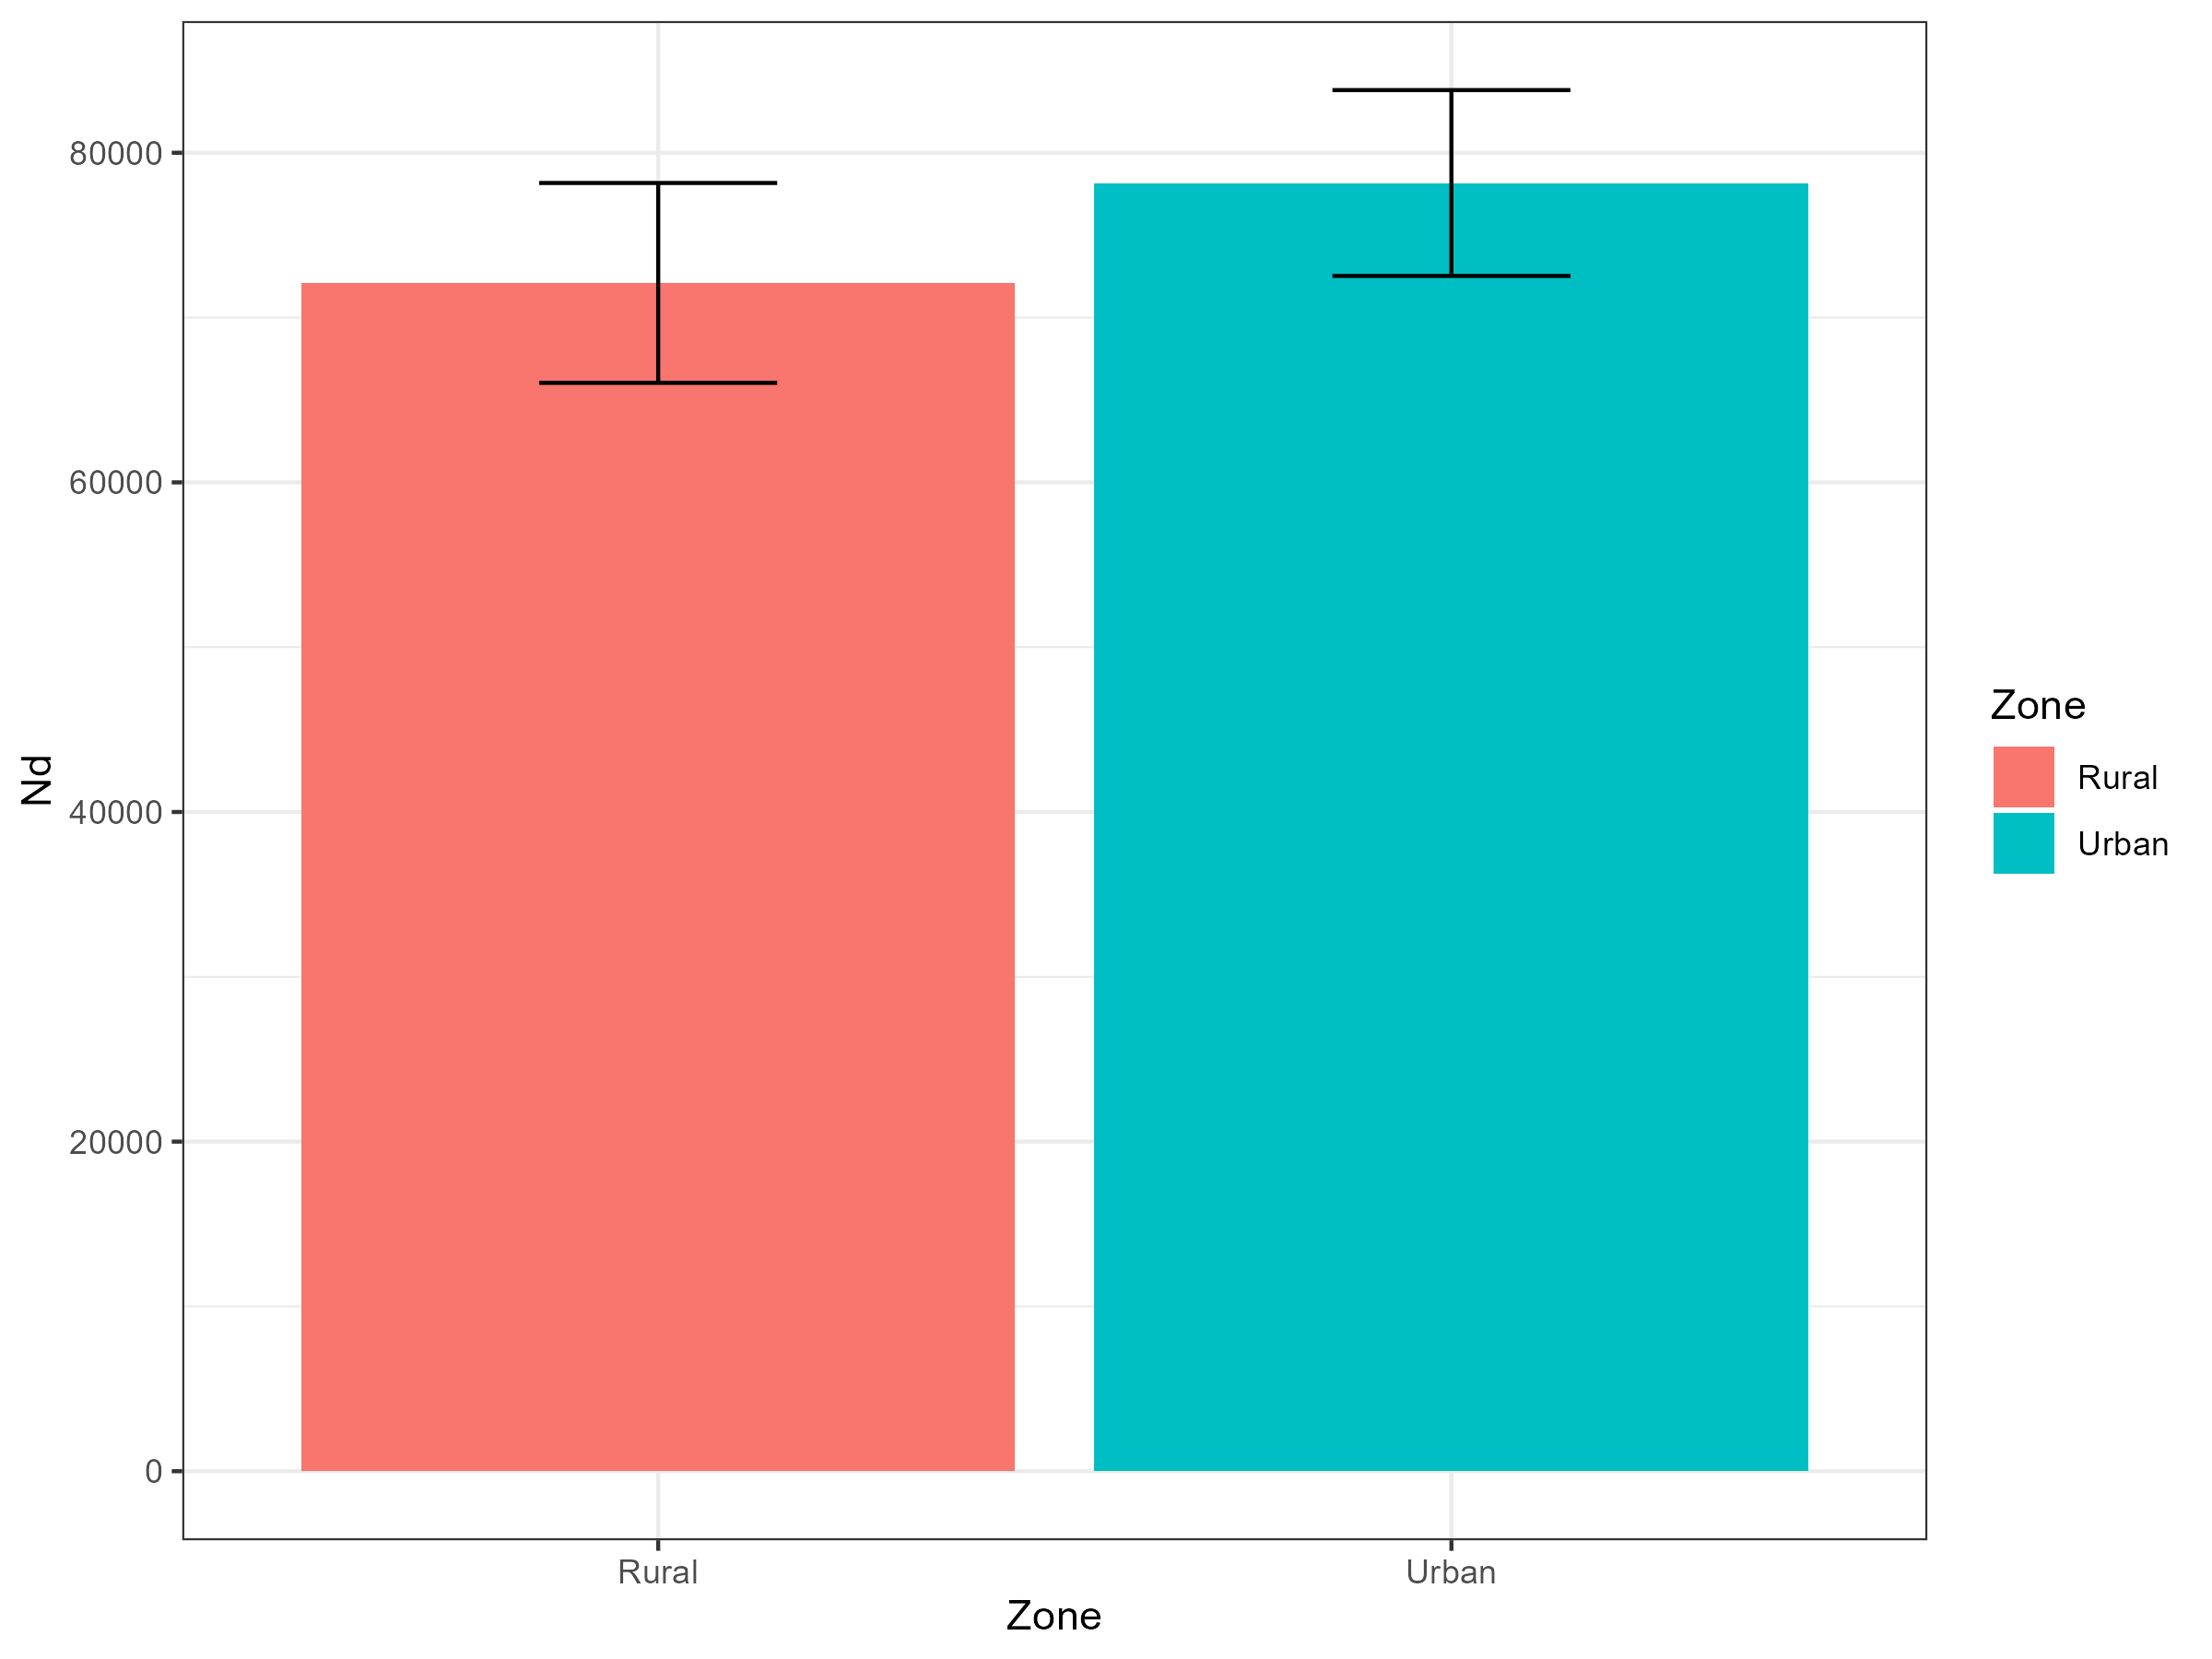
\includegraphics[width=33.33in]{www/05_graficas/03_bar_pers} \caption{Distribution of Population Income}\label{fig:barIncome}
\end{figure}

\begin{longtable}[]{@{}
  >{\raggedright\arraybackslash}p{(\columnwidth - 8\tabcolsep) * \real{0.1944}}
  >{\raggedright\arraybackslash}p{(\columnwidth - 8\tabcolsep) * \real{0.2222}}
  >{\raggedright\arraybackslash}p{(\columnwidth - 8\tabcolsep) * \real{0.1944}}
  >{\raggedright\arraybackslash}p{(\columnwidth - 8\tabcolsep) * \real{0.1944}}
  >{\raggedright\arraybackslash}p{(\columnwidth - 8\tabcolsep) * \real{0.1944}}@{}}
\caption{Population distribution by area}\tabularnewline
\toprule\noalign{}
\begin{minipage}[b]{\linewidth}\raggedright
Zone
\end{minipage} & \begin{minipage}[b]{\linewidth}\raggedright
Number of Individuals (Nd)
\end{minipage} & \begin{minipage}[b]{\linewidth}\raggedright
Standard Error (Nd\_se)
\end{minipage} & \begin{minipage}[b]{\linewidth}\raggedright
Lower Limit (Nd\_low)
\end{minipage} & \begin{minipage}[b]{\linewidth}\raggedright
Upper Limit (Nd\_upp)
\end{minipage} \\
\midrule\noalign{}
\endfirsthead
\toprule\noalign{}
\begin{minipage}[b]{\linewidth}\raggedright
Zone
\end{minipage} & \begin{minipage}[b]{\linewidth}\raggedright
Number of Individuals (Nd)
\end{minipage} & \begin{minipage}[b]{\linewidth}\raggedright
Standard Error (Nd\_se)
\end{minipage} & \begin{minipage}[b]{\linewidth}\raggedright
Lower Limit (Nd\_low)
\end{minipage} & \begin{minipage}[b]{\linewidth}\raggedright
Upper Limit (Nd\_upp)
\end{minipage} \\
\midrule\noalign{}
\endhead
\bottomrule\noalign{}
\endlastfoot
Rural & 72,102 & 3,062 & 66,039 & 78,165 \\
Urban & 78,164 & 2,847 & 72,526 & 83,802 \\
\end{longtable}

\hypertarget{histograms}{%
\section{Histograms}\label{histograms}}

Histograms serve to present the distribution of a single numeric (continuous) survey variable or response. If one had a census, then the histogram is a powerful tool to describe the underlying distribution, even for very large datasets. When displaying sample data, however, the sampling weights must be taken into account when estimating frequencies or relative frequencies of population units having values in the specified histogram bins. Modern survey analysis tools can easily provide weighted histograms where the sampling weights are incorporated.

Histograms are the precursors to density function estimates, and the later can be thought of as histograms with very large number of bins. The \texttt{survey} package in R provides functions that can plot smoothed density estimates obtained accounting for the sampling weights.

\hypertarget{graphical-analysis-with-survey-tools}{%
\subsection{Graphical Analysis with Survey Tools}\label{graphical-analysis-with-survey-tools}}

Once the database containing the sample is available and the sampling design has been defined, initial visual analyses can be conducted. It is recommended to begin with graphical analyses that, thanks to the principle of representativeness, reflect the behavior of continuous variables not only in the obtained sample but also in the study population, using sampling weights for sample expansion.

A common example of visualization in this type of analysis is the use of histograms to represent the distribution of variables such as income. These charts allow us to observe the distribution of the variable of interest in the expanded population and to understand its shape, dispersion, and general trends.

It is also common to perform graphical analyses broken down by subgroups, such as geographic areas (urban and rural) or thematic characteristics like gender (male and female). This approach helps identify key differences among specific population subgroups, for instance, by examining income distribution in men and women over the age of 18. Such breakdowns help visualize and communicate potential gaps between subgroups of interest.

In this way, charts help to communicate results in an accessible manner, offering a clear and straightforward visual representation for audiences who may not be familiar with the technical details of estimation methods.

In \ref{fig:histIncome} the horizontal axis (x) represents income levels, spanning from 0 to over 4000 monetary units, while the vertical axis (y) indicates frequency, meaning the number of individuals within each income range.

The distribution shows that most of the population is concentrated at lower income levels, with a particularly high frequency near 0. As income levels rise, frequency declines sharply, indicating a right-skewed (positively skewed) distribution with a smaller proportion of people at higher income levels. The light gray bars visually emphasize this concentration at lower incomes, highlighting a significant disparity in the population's income distribution.

\begin{figure}
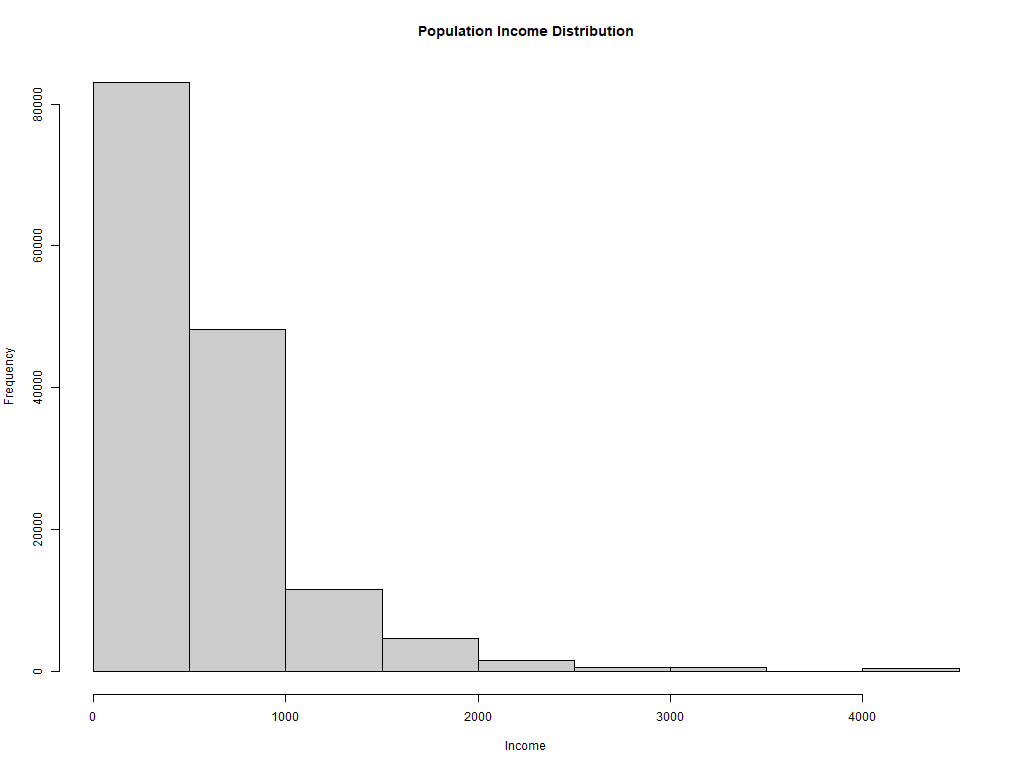
\includegraphics[width=14.22in]{www/05_graficas/01_hist_ingreso} \caption{Distribution of Population Income}\label{fig:histIncome}
\end{figure}

As an example, Figure \ref{fig:HistIncomeExpenditureSex} presents two histograms illustrating the distribution of income and expenditure by sex. In the histogram on the left, titled ``Income Histograms by Sex,'' we observe the income distribution, where blue bars represent men and pink bars represent women. The majority of the population, both male and female, is concentrated in the lower income levels, showing a right-skewed distribution. In the lower income levels, there are more men than women, while at higher income levels, the difference is less pronounced.

In the histogram on the right, titled ``Expenditure Histograms by Sex,'' the distribution of expenditure is shown, also broken down by sex. Similar to income, most of the population of both sexes is concentrated in the lower expenditure levels, with a right-skewed trend. There is also a higher proportion of men in the lower expenditure levels, while at higher levels, the representation between sexes is more balanced. These histograms exemplify the similarity in the income and expenditure distributions between men and women, although men appear to be slightly more represented in the lower levels of both variables.

\begin{figure}
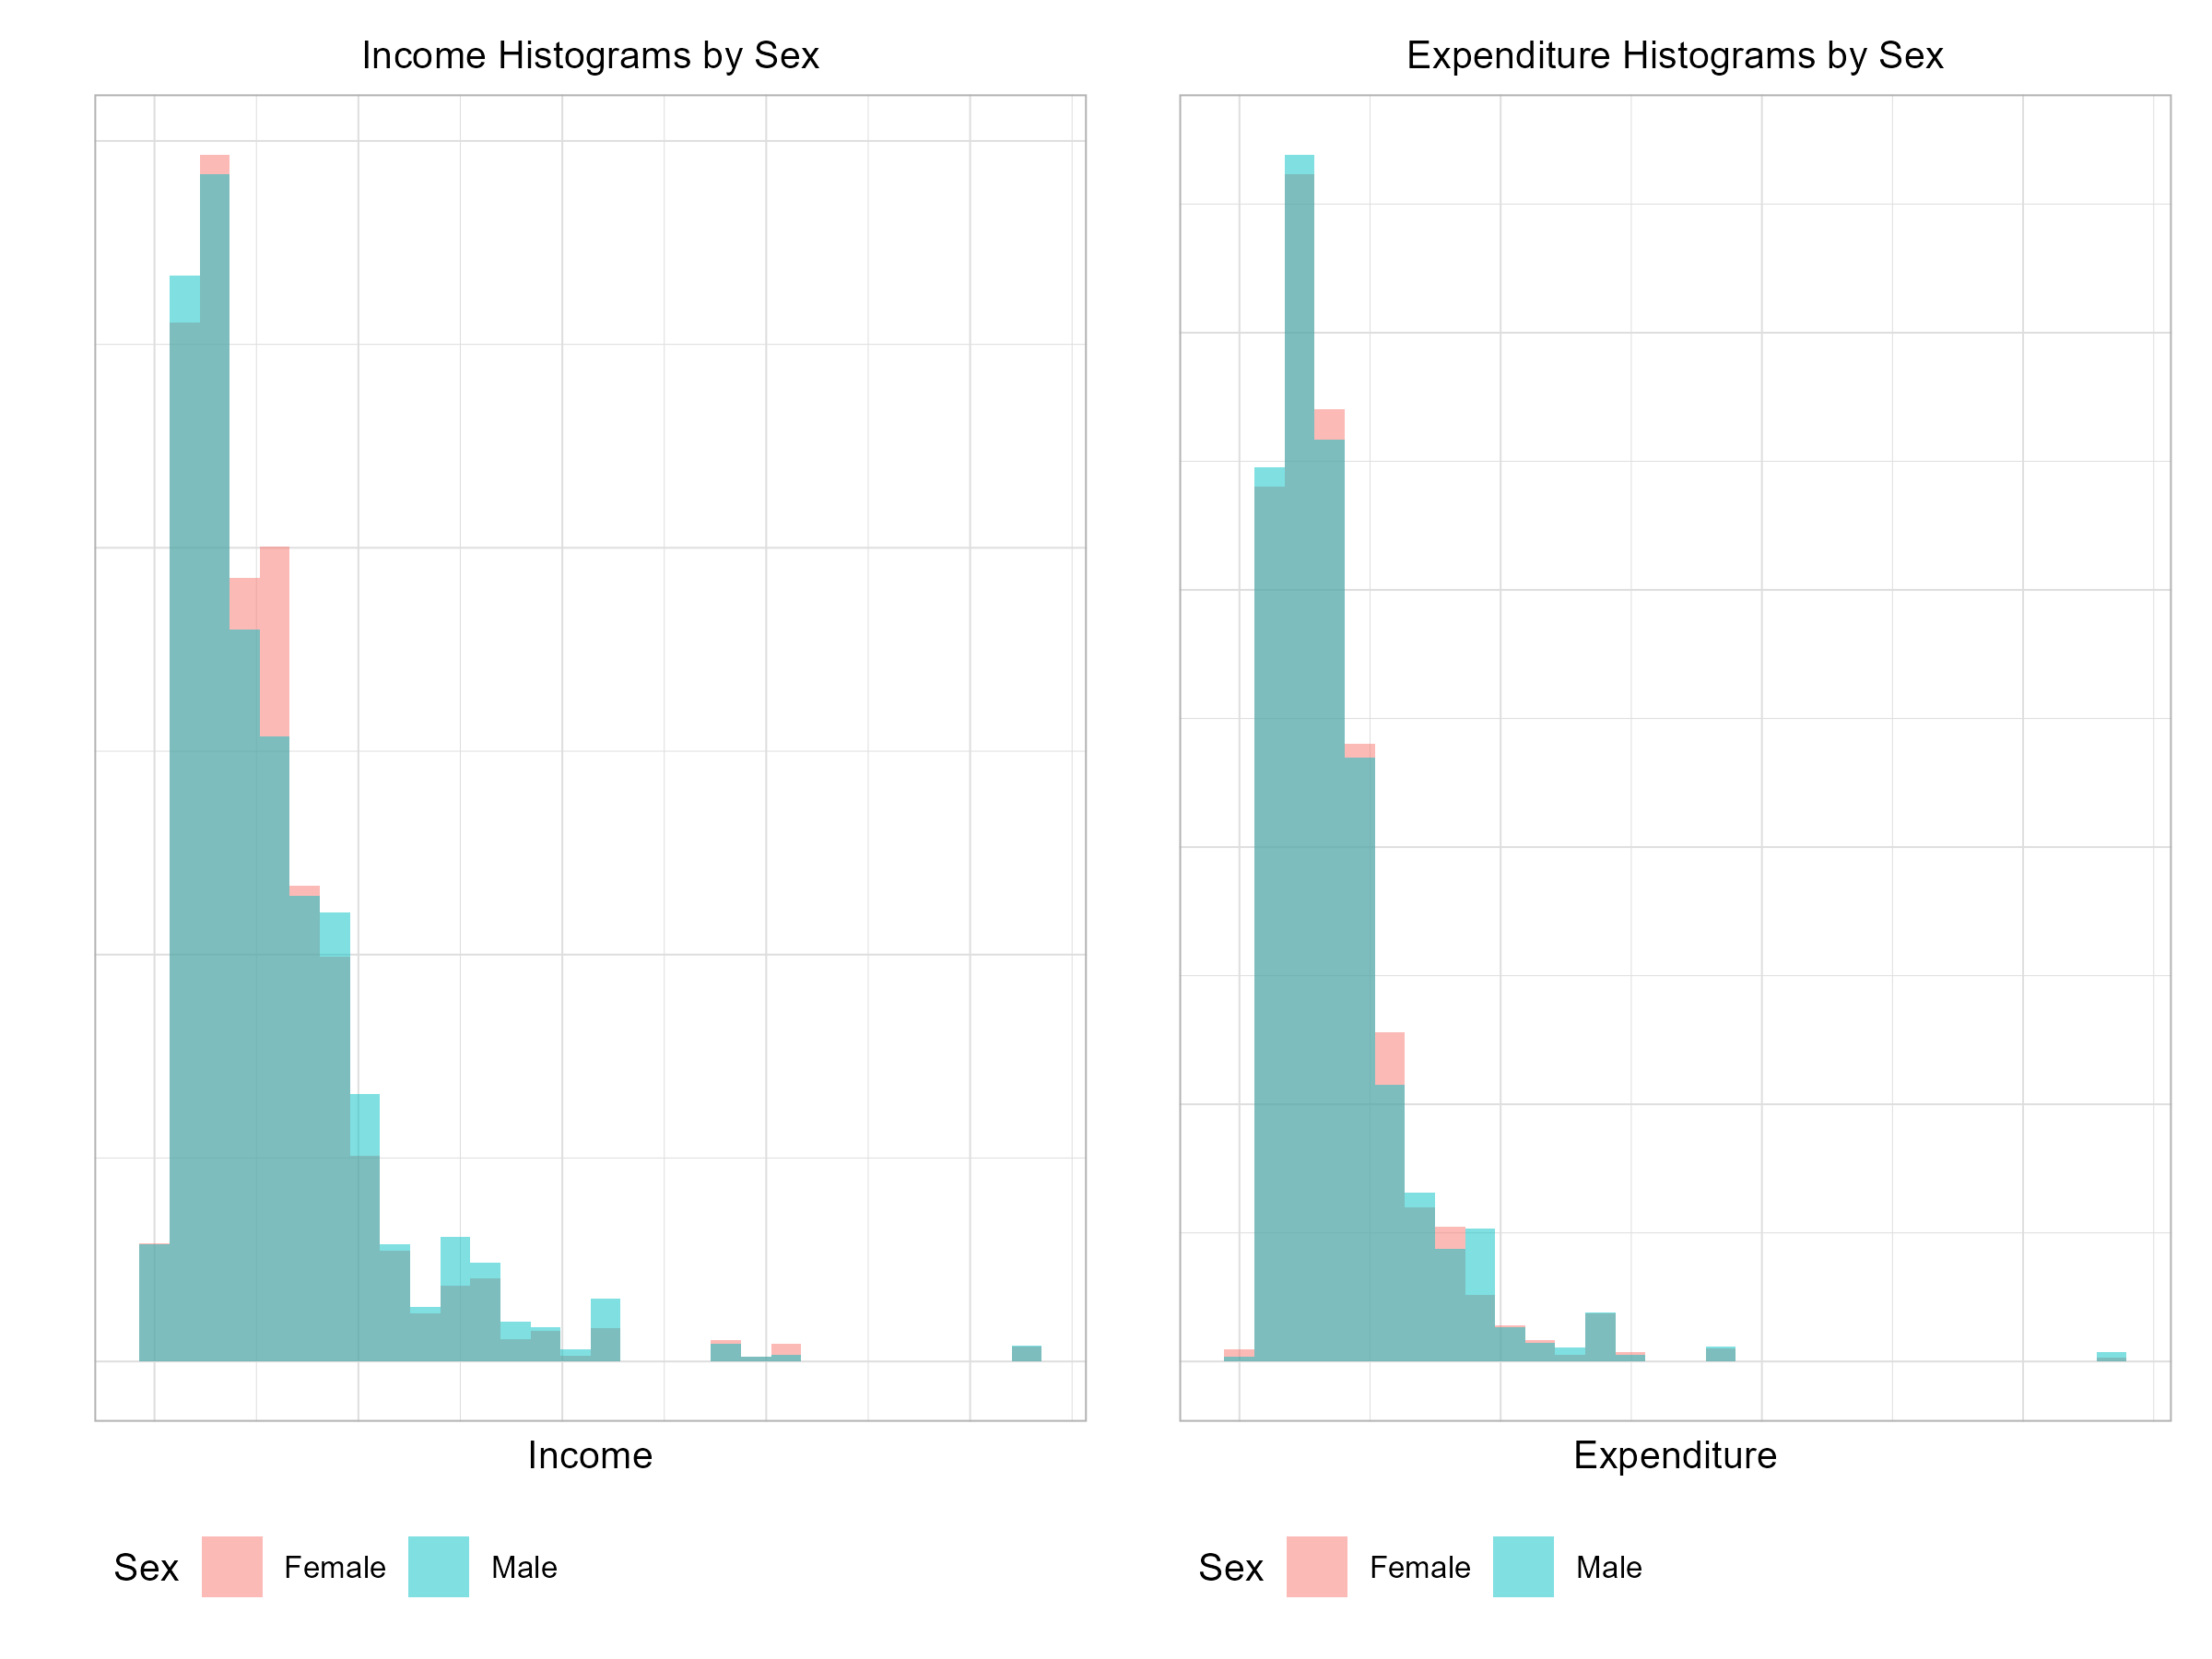
\includegraphics[width=33.33in]{www/05_graficas/02_Hist_sex} \caption{Histograms of Income and Expenditure by Sex}\label{fig:HistIncomeExpenditureSex}
\end{figure}

\hypertarget{box-plots}{%
\section{Box Plots}\label{box-plots}}

Box plots are often used to present the distribution of continuous variables. They can summarize large datasets by providing a visual display providing easy visual to identify location, range, variability and outliers. They are great also for enabling comparing distributions across specified grouping variables, such as strata, clusters, etc.

The key to producing such graphs from complex sample surveys is to account for the sampling weights when estimating the location measures that drive the plot, namely the quartiles. Once these have been estimated using the methods described earlier, the resulting box plots will be good depictions enabling analysis of the underlying population distributions.

\hypertarget{scatter-plots}{%
\section{Scatter Plots}\label{scatter-plots}}

Scatter plots are the tool of choice to explore relationships between two continuous variables, potentially revealing patterns or trends in the data. These plots face the two challenges discussed above. First one needs to try and convey in the plot that the different sample observations carry different weights. For small to moderate sample sizes this can be done by plotting circles or dots of varying sizes where the symbol size represents the corresponding observation sampling weight. Plots like these can be obtained using standard bubble plot tools or the scatter plot available in the \texttt{survey} package in R.

The second challenge, present when there is a large dataset to be displayed, has motivated creation of some alternatives. Two ideas are worth noting. The first one is subsampling. One may choose to select a small to moderate subsample from the full dataset to display. Such a sample should be selected with replacement and with probabilities proportional to the observations sampling weights. Then the resulting smaller dataset can be used to produce a standard scatter plot. The subsample obtained in this way behaves approximately as a simple random sample from the survey population - see \citet{Lumley2010} page 69.

The other alternative is to produce so-called \emph{hexagonal binned scatter plots}. This involves dividing the plot surface into a grid of hexagons and combining all the points that fall into a grid cell into a single plotted hexagon whose shading or size indicates the number of points in the bin. With complex household survey data, the number of points in a hexagonal bin should be replaced by the sum of the weights for points in the bin - see \citet{Lumley2010} page 70.

The third alternative is to avoid the display of the individual data points altogether, but instead produce \emph{smoothed scatter plots}. One idea that can be useful would be to estimate specified quantiles (say the quartiles) of the y-axis (response) variable conditional on the values of the x-axis (predictor) variable, and smooth these across the range of the x-axis. Such plots can easily signal whether the y-variable has any relationship with the x-variable, and suggest the kind of curves that might be useful in summarising or modelling such a relationship - see \citet{Lumley2010} page 71.

As an example in \ref{fig:ScatterIncome}, the following scatterplot is presented, showing the weighted relationship between income and expenditure in a population. In this plot, the size of the points represents the weight assigned to each observation. A high concentration of points is observed at lower income and expenditure levels, suggesting that most of the population has low income and low expenditure. Although there is an upward trend, indicating that income and expenditure tend to increase together, the dispersion of points reveals that higher expenditure is not always associated with proportionally higher income. Some larger points, corresponding to observations with greater weight, are distributed across different levels of income and expenditure without concentrating in a single area. Additionally, a few isolated points at high expenditure levels may represent outliers with considerably higher-than-average expenditure. Overall, this plot suggests a positive relationship between income and expenditure, accompanied by significant variability and some exceptional cases.

\begin{figure}
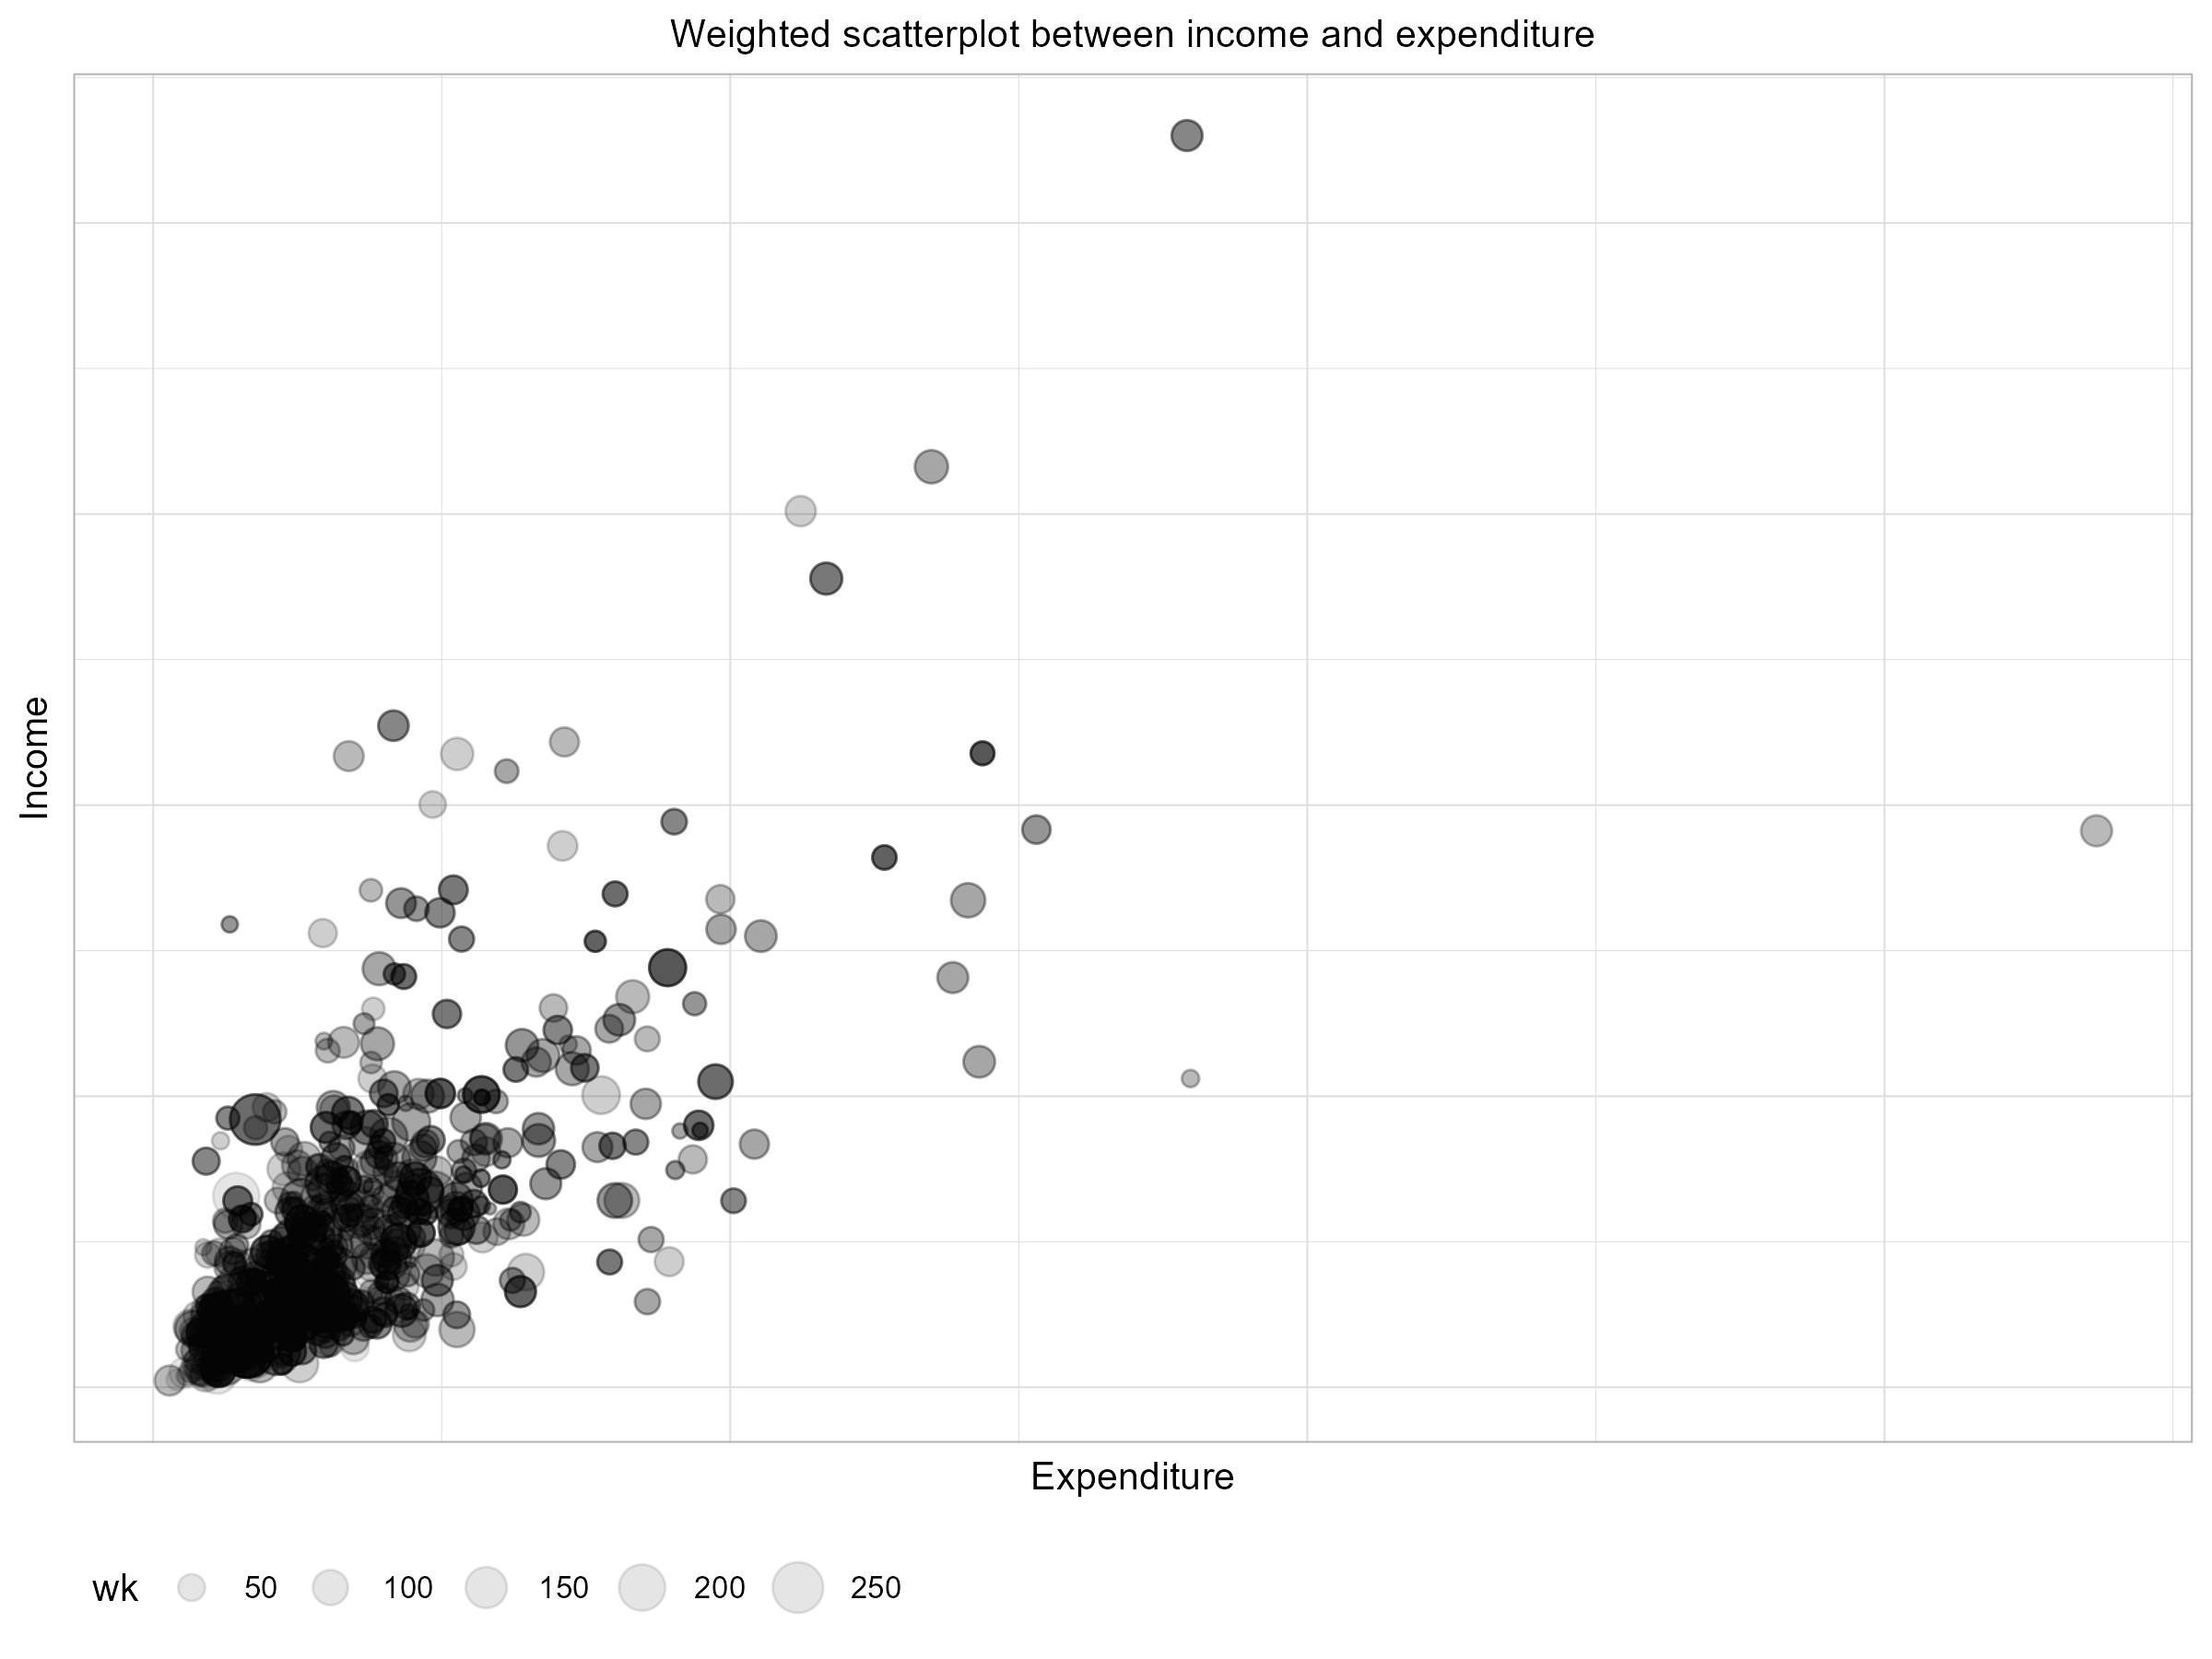
\includegraphics[width=33.33in]{www/05_graficas/02_scatterplot_ingreso_gasto} \caption{Weighted scatterplot between income and expenditure}\label{fig:ScatterIncome}
\end{figure}

\hypertarget{maps}{%
\section{Maps}\label{maps}}

Maps are the display of choice to present the behavior of the interest variable across geographical domains. Maps that aim to present how a single response variable behaves can be easily obtained by plotting a summary of the response across the domains. Such a summary (say mean or median) should be an estimate for the corresponding population parameter btained accounting for the sample design and weights.

Secondary survey analysts will may find that the limits of what mapping they can do is the level of geographic detail provided with the survey microdata. Many household sample surveys are design to provide precise estimates at some broad geographic level, say the country or its first level geographic subdivisions, such as states or departments. Lower level geographies are seldom disseminated with the survey microdata due to confidentiality protection constraints imposed.

It is therefore important that statistical agencies conducting the household sample surveys and preparing the dissemination of the corresponding microdata consider carefully which level of geographic detail may be included with public use datasets.

One area which still needs further research is that of providing appropriate means to convey the uncertainty of underlying point estimates when mapping these.

\hypertarget{nso-practical-example-3}{%
\section{NSO -- Practical example}\label{nso-practical-example-3}}

In this subsection we will include the experience of a NSO on displaying information through graphics.

\hypertarget{other-modeling-scenarios}{%
\chapter{Other modeling scenarios}\label{other-modeling-scenarios}}

In this section we indicate the literature and software supporting the fitting of some other models to complex household survey data, including:

\hypertarget{multilevel-models}{%
\section{Multilevel models}\label{multilevel-models}}

Multilevel models, also known as mixed effects models or hierarchical models, are a statistical technique used in the analysis of household survey data to incorporate a hierarchical or multilevel structure. In these surveys, data are collected at the individual level (e.g., information about the age, gender, and education of each household member) and at the household level (e.g., household income, home ownership, and geographic location). Additionally, these models allow for the analysis of how household-level and individual-level factors influence responses to survey questions. For example, a multilevel model could be used to investigate how household income and the ages of household members influence the consumption of healthy foods.

In multilevel models, two types of effects are considered: fixed effects and random effects. Fixed effects represent the average relationships between variables, while random effects model the variation in these relationships across households. Thus, multilevel models account for heterogeneity in the population and provide more accurate estimates of the variables of interest. Therefore, multilevel models are a valuable tool in analyzing household survey data, as they allow for the examination of how both household-level and individual-level factors influence survey responses, while accounting for the hierarchical structure of the data.

Relevant references on the use of multilevel models in household surveys include \citet{goldstein2011}, a classic reference for multilevel data analysis that discusses the use of hierarchical models in various contexts, including household surveys; \citet{gelmanhill2019}, which offers an accessible introduction to the theory and practice of hierarchical models; \citet{rabe2012multilevel}, a practical guide for analyzing multilevel and longitudinal data using statistical software such as Stata; and \citet{browne2006comparison}, which compares Bayesian and frequentist approaches based on likelihood.

\hypertarget{model-with-random-intercept}{%
\subsection{Model with Random Intercept}\label{model-with-random-intercept}}

In the analysis of multilevel models, two types of estimates are relevant. The first is associated with the regression coefficients, generally referred to as the fixed parameters of the model; the second pertains to the variance estimates, usually called the random parameters of the model. Any multilevel regression analysis should always begin with estimating the variance at both levels for the dependent variable.

The recommended first step in multilevel regression analysis involves decomposing the variance of the dependent variable across the different levels. For example, assuming that the variable of interest is individual income and that there is a hierarchical relationship between individuals and strata, the variance of income can be decomposed into two parts: the variance within strata and the variance between strata. These two components of variance can be obtained from a simple multilevel regression with a null model represented by the following expression:

\[
y_{ij} = \beta_{0j} + \epsilon_{ij}
\]

Here, \(y_{ij}\) represents the income of individual \(i\) in stratum \(j\); \(\beta_{0j}\) is the intercept in stratum \(j\); \(\epsilon_{ij}\) is the residual for individual \(i\) in stratum \(j\); \(\gamma_{00}\) is the overall intercept, and \(\tau_{0j}\) is the random effect for the intercept. For this model, it is assumed that:

\[
\tau_{0j} \sim N(0, \sigma_{\tau}^{2})
\]

Additionally,

\[
\epsilon_{ij} \sim N(0, \sigma_{\epsilon}^{2}).
\]

According to \citet{cai2013investigation}, there is sufficient evidence that sampling weights should be used in multilevel modeling to obtain unbiased estimates. Currently, different authors recommend various approaches on how to use sampling weights in hierarchical models. For instance, \citet{pfeffermann1998weighting} and \citet{asparouhov2006general} advise employing a pseudolikelihood approach to calculate estimates within and between different levels to achieve unbiased estimates.

An important concept in this type of analysis is the intra-class correlation (ICC), which refers to the proportion of the total variance of a variable that is explained by differences between groups or levels (strata) in the model. In other words, the ICC measures the similarity or correlation between observations within the same group or level compared to observations from different groups. This quantity is calculated as follows:

\[
\rho = \frac{\sigma_{\tau}^{2}}{\sigma_{\tau}^{2} + \sigma_{\epsilon}^{2}}
\]

A high ICC indicates that a large proportion of the total variation in the variable is due to differences between groups, suggesting that the groups are distinct from one another and that the group effects should be considered in the model. Conversely, a low ICC indicates that most of the variation in the variable occurs within groups, implying that the group effects are not as significant in explaining variability in the variable.

\hypertarget{model-with-random-slope}{%
\subsection{Model with Random Slope}\label{model-with-random-slope}}

This type of model allows the relationship between the independent variable and the dependent variable to change according to some other explanatory variable. In other words, it permits the slope of the relationship between the variables to differ as groups or subsets of data are considered. In a simple linear regression model, the relationship is modeled as a straight line with a fixed slope. However, in a model with a random slope, the slope can vary according to another explanatory variable.

In these types of models, the relationship between the variables can imply a curve with different slopes for different subgroups. Random slope models are useful in situations where it is expected that the relationship between the variables changes in a nonlinear way or when differences in slope among subgroups need to be modeled. Consider the following model:

\[
Income_{ij} = \beta_{0} + \beta_{1j} Spending_{ij} + \epsilon_{ij}
\]

where \(\beta_{1j}\) is given as

\[
\beta_{1j} = \gamma_{10} + \gamma_{11} Stratum_{j} + \tau_{1j}
\]

In this particular case, the slope varies according to the sampling strata, while the intercept remains fixed. This allows for a more accurate capture of how the relationship between spending and income may differ across different groups, providing a better understanding of the patterns in the data.

\hypertarget{model-with-random-intercept-and-slope}{%
\subsection{Model with Random Intercept and Slope}\label{model-with-random-intercept-and-slope}}

Models with random intercepts and slopes are a type of statistical model that allows for modeling the relationship between a response variable and one or more predictor variables, considering both fixed and random effects. In these models, the regression coefficients (i.e., the slope and intercept) are treated as random rather than fixed, meaning these coefficients can vary across units of analysis, which may be individuals, groups, geographical regions, etc. These variations are modeled as random effects incorporated into the regression equation.

Continuing with the context of a household survey, consider the following model:

\[
Income_{ij} = \beta_{0j} + \beta_{1j} Spending_{ij} + \epsilon_{ij}
\]

where the intercept and slope are modeled as:

\[
\beta_{0j} = \gamma_{00} + \gamma_{01} Stratum_{j} + \tau_{0j}
\]

and

\[
\beta_{1j} = \gamma_{10} + \gamma_{11} Stratum_{j} + \tau_{1j}
\]

In this model, \(\beta_{0j}\) and \(\beta_{1j}\) depend on the stratum variable, allowing both the intercept and slope to change according to the group of interest. This provides greater flexibility and better captures the heterogeneity in the data, reflecting how relationships between the variables may differ across subgroups.

\hypertarget{survival-models}{%
\section{Survival models}\label{survival-models}}

\hypertarget{loglinear-models-for-contingency-tables}{%
\section{Loglinear models for contingency tables}\label{loglinear-models-for-contingency-tables}}

When analyzing the relationships between variables that generate estimated totals in a contingency table (a rectangular arrangement that organizes data based on two or more categorical variables, showing the frequency or proportion of cases falling into each combination of categories), it is possible to use a log-linear model. This type of model is used to study the association between categorical variables while controlling for or considering potential effects of other covariates. Additionally, it allows for adjusting the observed associations in the contingency table and assessing whether these associations are statistically significant.

Log-linear models in contingency tables can be used to determine whether there is a significant association between categorical variables; adjust the association between variables of interest by accounting for other variables that may influence the relationship; evaluate how the probability of a category in one categorical variable changes given a change in another categorical variable; and estimate the probability of a case falling into a specific category of a categorical variable given the information from other variables.

The term log-linear essentially describes the role of the link function used in generalized linear models. In the simplest case, with two categorical variables inducing data from counts or proportions in contingency tables, the following statistical model can be formulated:

\[
\ln(\pi_{ijk}) = \mu + \lambda_i^X + \lambda_j^Y + \lambda_{ij}^{XY},   
\]

where \(\pi_{ijk}\) is the conditional probability of occurrence for the combination of categories \(i\) and \(j\) in the categorical variables \(X\) and \(Y\), respectively; \(\mu\) is the intercept representing the logarithm of the reference probability; \(\lambda_i^X\) and \(\lambda_j^Y\) are the main effects associated with categories \(i\) and \(j\) in the variables \(X\) and \(Y\), respectively; and finally, \(\lambda_{ij}^{XY}\) is the interaction effect between categories \(i\) and \(j\) in the categorical variables. The natural logarithm function is commonly used in these models to transform conditional probabilities and allow for interpretation in terms of log-odds. In summary, the model describes how the conditional probabilities of categorical events are related to each other and how these relationships can be influenced by main and interaction effects in the categorical variables \(X\) and \(Y\).

This statistic is applied after a statistical model has been chosen (such as simple linear regression, logistic regression, among others). The Wald chi-squared test statistic for the null hypothesis of independence between rows and columns in a contingency table is defined as follows:

\[
Q_{wald} = \hat{\boldsymbol{Y}}^{t} \left(\boldsymbol{H} \hat{\boldsymbol{V}} \left(\hat{\boldsymbol{N}}\right) \boldsymbol{H}^{t}\right)^{-1} \hat{\boldsymbol{Y}}
\]

where

\[
\hat{\boldsymbol{Y}} = \left(\hat{N} - E\right)
\]

is a vector of \(R \times C\) differences between observed and expected cell counts, that is, \(\hat{N}_{rc} - E_{rc}\). The matrix \(\boldsymbol{H} \hat{\boldsymbol{V}} \left(\hat{\boldsymbol{N}}\right) \boldsymbol{H}^{t}\) represents the estimated variance-covariance matrix for the difference vector. In the case of a complex survey design, the variance-covariance matrix of the weighted frequency counts, \(\hat{V} \left(\hat{N}\right)\), is estimated using resampling methods or Taylor approximation. The matrix \(\boldsymbol{H}\) is the inverse of the matrix \(\boldsymbol{J}\) given by:

\[
\boldsymbol{J} = -\left[\frac{\delta^{2} \ln PL\left(\boldsymbol{B}\right)}{\delta^{2} \boldsymbol{B}}\right] \bigg|_{\boldsymbol{B} = \hat{\boldsymbol{B}}}
\]

Under the null hypothesis of independence, the Wald statistic follows a chi-squared distribution with \((R-1) \times (C-1)\) degrees of freedom:

\[
Q_{wald} \sim \chi^{2}_{(R-1)(C-1)}
\]

The F transformation of the Wald statistic is:

\[
F_{wald} = Q_{wald} \times \frac{df - (R-1)(C-1) + 1}{(R-1)(C-1) df} \sim F_{(R-1)(C-1), df - (R-1)(C-1) + 1}
\]

\hypertarget{tables}{%
\chapter{Tables}\label{tables}}

\emph{Tables} form a key component regarding how agencies disseminate statistics from household survey data. Using tables efficiently helps minimize the amount of numeric values presented within the text, and to organise the survey results for presentation to the users and wider audiences. It is therefore important to discuss some core principles and ideas to the preparation and production of tables with survey results.

Before we enter detailed discussions, it is important to distinguish three main types of tables that can be used for presenting the results of a survey:

\begin{itemize}
\item
  presentation tables;
\item
  reference tables;
\item
  long / database like tables.
\end{itemize}

The guidelines for each of these kinds of tables will be somewhat different, though all three types should follow some key principles, as suggested by Miller (2004), namely:

\begin{itemize}
\item
  \textbf{Principle 1.} Make it easy for your reader to find and understand the numbers presented in your tables;
\item
  \textbf{Principle 2.} Draw the layout and labels of the table in a simple and direct way, helping to focus attention on the results you want to show.
\end{itemize}

\hypertarget{presentation-tables}{%
\section{Presentation tables}\label{presentation-tables}}

These are generally small tables, used to highlight certain key results obtained from the survey, to be presented in press releases, executive summaries, scientific articles or reports, or on landing web pages which contain the survey output. They are not expected to provide all results on a topic, but rather to highlight key results that should draw the attention of a reader to some of the main stories the data have produced.

In presentation tables, the data should be presented concisely, and organized to support the text with the analysis of the corresponding data. They should be designed in such a way to help readers learn about the key results on the topic provided by the survey.

Short, well-designed and formatted tables can provide a lot of information that readers can absorb quickly. This applies to tables published in any vehicle: reports, press releases, articles, electronic publications or websites. The example below illustrates the idea.

Presentation tables should have rows (and possibly columns) sorted in a way that helps the reader perceive patterns, such as high or low figures. Such tables will often sacrifice detail in exchange for readability and understanding. Numbers should be presented with no more than 3 or 4 digits altoghether. If they area population counts, use thousands. If the figures are percentages, use no more than a single decimal digit, or even present only percentages rounded to the nearest integer, if the precision of the estimates do not warrant providing decimals (e.g.~margins of error larger than 1\%).

\hypertarget{example-of-presentation-table-and-corresponding-text---include-in-a-box.}{%
\section{Example of presentation table and corresponding text - include in a box.}\label{example-of-presentation-table-and-corresponding-text---include-in-a-box.}}

Among middle and senior managers, women are outnumbered at all ages. The underrepresentation of women was observed in all age groups. Relative to their share among non-managers, women were outnumbered among middle and senior managers. In all age groups, women accounted for about 4 in 10 middle managers and 3 in 10 senior managers.

Table 2 - Share of women (\%) by age group and occupation

\begin{longtable}[]{@{}cccc@{}}
\toprule\noalign{}
Age group & Non-managers & Middle managers & Senior managers \\
\midrule\noalign{}
\endhead
\bottomrule\noalign{}
\endlastfoot
25 to 34 years & 44.6 & 40.3 & 28.4 \\
35 to 44 years & 45.7 & 38.7 & 31.3 \\
45 to 54 years & 48.3 & 40.5 & 31.7 \\
\end{longtable}

Note: The category ``women'' includes women, as well as some non-binary people. Source: Statistics Canada, Census of Population, 2021. \url{https://www150.statcan.gc.ca/n1/pub/36-28-0001/2024010/article/00005-eng.htm}

\hypertarget{reference-tables}{%
\section{Reference tables}\label{reference-tables}}

These are longer tables, generally used to present more complete sets of results from statistical studies. They should be limited in size to something that could be contained in a few pages of a printed report, say, with a number of rows no larger than 200, and no more than say 12 columns. Anything bigger than that should be considered for dissemination as a \emph{database like table}, probably available only for download from a website or readable from some digital media.

Reference tableswill typically take core classification, domain definition or \emph{explanatory} variables to define the rows, and have the \emph{outcome} classification or output variables define the columns. In both directions, sorting should typically be such that it is easier for the readers to locate the data that they are most interested in, either using alphabetic or well known classifications.

Reference tables have in many cases been replaced by access to interactive databases that allow the interested user to obtain the tables they want from a website.

Tables (of all types) should be \emph{self-sustaining}. The idea is that each table should have the necessary metadata, so that if copied from one location to another it still makes sense. If you can get your tables to be \emph{self-sustaining}, they will be easier to understand correctly, either in or out of the original context.

Anatomy of a table. Figure XX presents the essential components of a table.

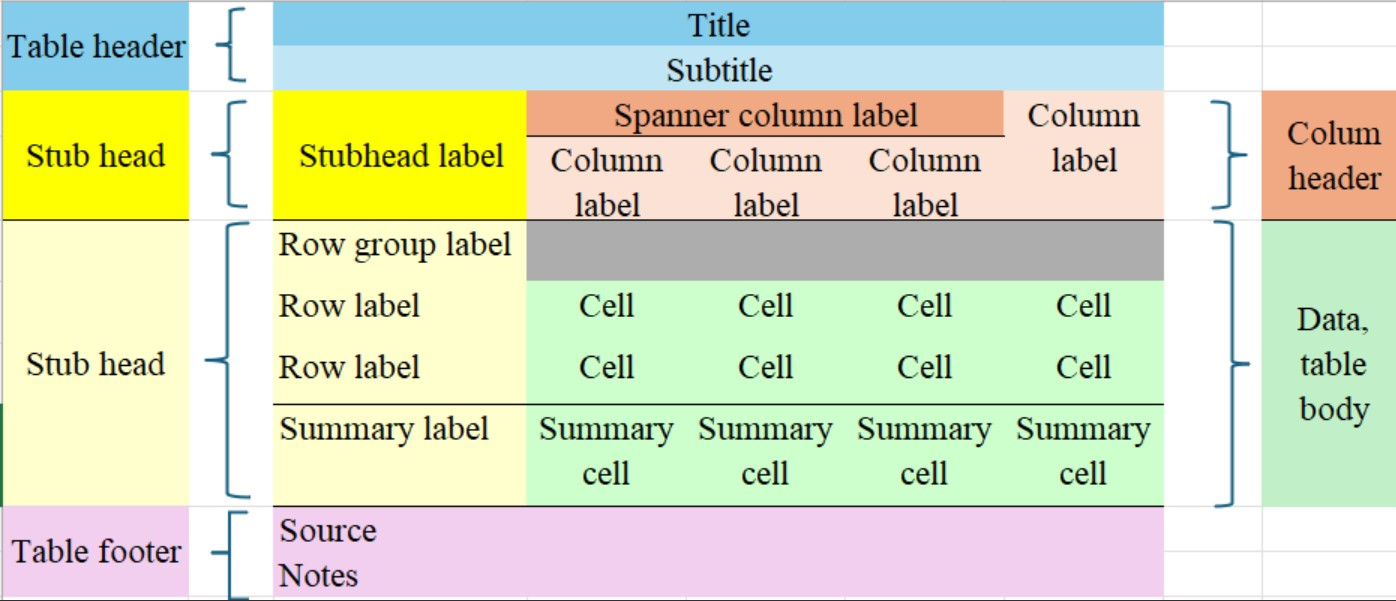
\includegraphics[width=0.5\textwidth,height=\textheight]{pics/Table1.jpg}

The title (and optional subtitle) of a table must provide a clear and precise indication of the data that will be presented in the table. These elements, combined, must answer the questions about what, where and when regarding the data to be presented inside the table. Be concise and avoid using verbs.

Column header elements should identify the data that is displayed in each column of the table. They must also provide much of the relevant metadata: unit of measurement, time period, geographical area, etc.

Stub elements, provided as the first column in the table, should identify the data that is displayed in each row of the table.

The source of the data must always be provided at the bottom of the table, and must indicate the organization responsible and the name of the survey or study that produced the results contained in the table. The omission of the citation of the source prevents the reader from seeking more information about the data presented, and should be avoided.

The Notes are optional, but they can be used to provide additional details about the data as needed to understand and use it correctly. Avoid using long texts, which if needed, would be better placed in a document that is then cited in the Notes section. If there is more than one Note, number sequentially, and use the numbers to indicate the corresponding calls inside the table. Make sure that the calls to Notes are sufficiently distinct from the actual figures / numbers inside te table to avoid confusion.

The Data is the most important piece of information that the user expects to get from the table. Therefore, it is essential to present them in a way that is easy to extract the relevant information. For some tables, depending on the message you want to convey, it may be easier to search for information by rows or columns. This should be the most important consideration when deciding whether to present the table in portrait or landscape orientation. Dividing lines, dotted lines, shading, and even spacing can be helpful in guiding the reader to read the table in the `right' direction.

Some basic rules for presenting the data include:

\begin{itemize}
\tightlist
\item
  Use similar spacing for columns whenever possible;
\item
  Avoid any unnecessary text;
\item
  The width of the table should be only the width necessary to present the data, and not the entire width of the available space;
\item
  Time series data should be presented in chronological order -- for reference tables, in ascending order; for presentation tables, this order can be reverse or descending to display the most recent data first;
\item
  Data on categorical variables should be presented using standard classifications; in reference tables, categories should be ordered according to the standard classification; in presentation tables, they can be presented in (descending) order of frequency to highlight the most frequent categories first;
\item
  Use as few decimal places as possible;
\item
  Use thousands separators; space is a better separator because it does not vary with the decimal separator according to language;
\item
  Always align the numbers to the right, ensuring that the decimal separator (comma or period, depending on the language) are aligned;
\item
  Never center the values unless they all have the same number of digits;
\item
  Do not leave blank cells on the table; missing values or `not applicable' situations must be identified with an appropriate symbol;
\item
  Round the data to units that make sense in each case; aim for providing 3 or 4 significant digits in presentation tables;
\item
  Rounding is also useful when the data is not very accurate, but be careful not to lose precision.
\end{itemize}

The recommendations provided here to reference tables should also apply to longer tables provided as databases, but these can have additional resources if they are embedded on websites. For example, there may be support for users to sort tables using the values in each column, which would be useful for large tables where the user may be looking for the higher (or lower) values in a given column.

\hypertarget{references}{%
\chapter*{References}\label{references}}
\addcontentsline{toc}{chapter}{References}

  \bibliography{chapterbib.bib}

\end{document}
